\documentclass{article}
\usepackage[a4paper,left=3cm,right=3cm,top=3cm,bottom=3cm]{geometry}
\usepackage[utf8]{inputenc}
\usepackage[T1]{fontenc}
\usepackage{latexsym,amsfonts,amsmath,amssymb,amstext,graphicx,titlesec,ae,aecompl,mathtools,tabularx, multirow, cancel, nicefrac,subcaption, blindtext, floatrow}
\setlength{\parindent}{0pt}
\newfloatcommand{capbtabbox}{table}[][\FBwidth]


\begin{document}

\begin{titlepage}
       \begin{center}
             \begin{huge}
				   %% Update assignment number here
                   \textbf{Assignment 5}
             \end{huge}
       \end{center}

       \begin{center}
             \begin{large}
                   Computational Intelligence, SS2020
             \end{large}
       \end{center}

       \begin{center}
 \begin{tabularx}{\textwidth}{|>{\hsize=.33\hsize}X|>{\hsize=.33\hsize}X|>{\hsize=.33\hsize}X|} 

                   \hline
                   \multicolumn{3}{|c|}{\textbf{Team Members}} \\
                   \hline
                   Last name & First name & Matriculation Number \\
                   \hline
                   Blöcher & Christian & 01573246 \\
                   \hline
                   Bürgener & Max & 01531577 \\
                   \hline
                    &  &  \\
                   \hline

             \end{tabularx}
       \end{center}
\end{titlepage}


\section{Classification - 2 dimensional feature}
\subsection{EM algorithm}

\begin{figure}[!ht]
	\makebox[\textwidth]{
	\begin{subfigure}{0.6\textwidth}
	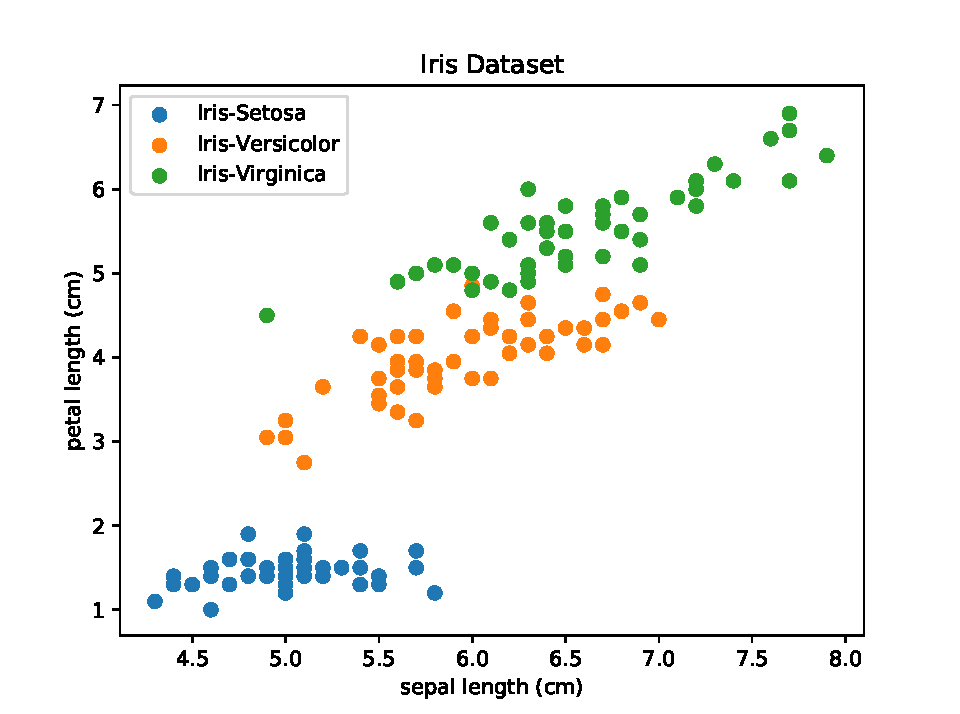
\includegraphics[width=\textwidth]{./Figures/data}
	%\caption{Dataset}
	\end{subfigure}
	\begin{subfigure}{0.6\textwidth}
	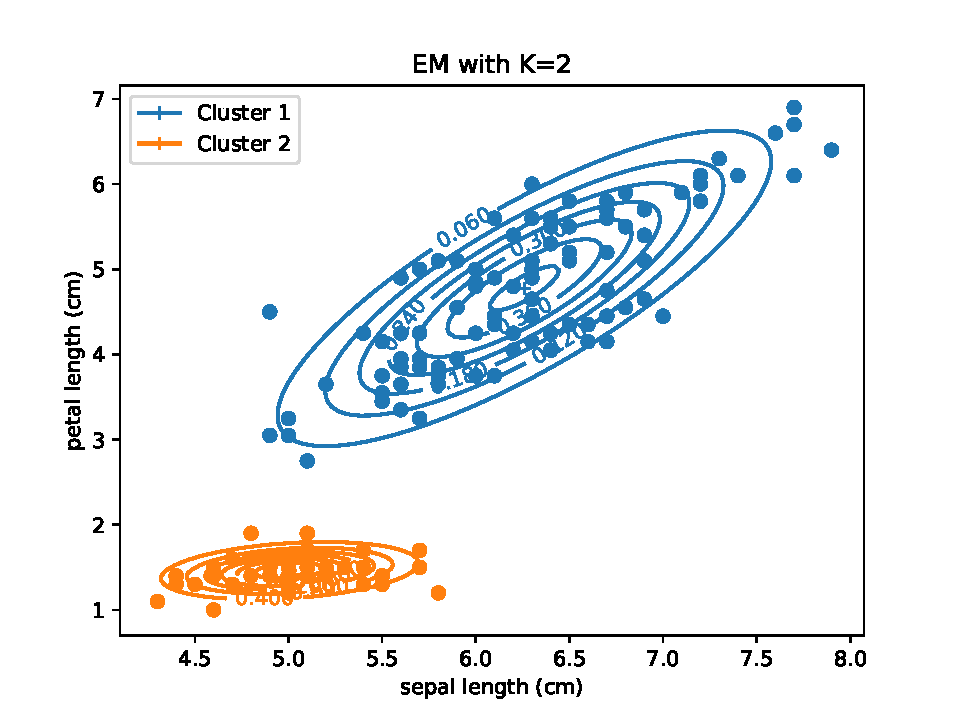
\includegraphics[width=\textwidth]{./Figures/2_1_EM_cont_K2}
	%\caption{$K=2$}
	\end{subfigure}
	}
	\makebox[\textwidth]{
	\begin{subfigure}{0.6\textwidth}
	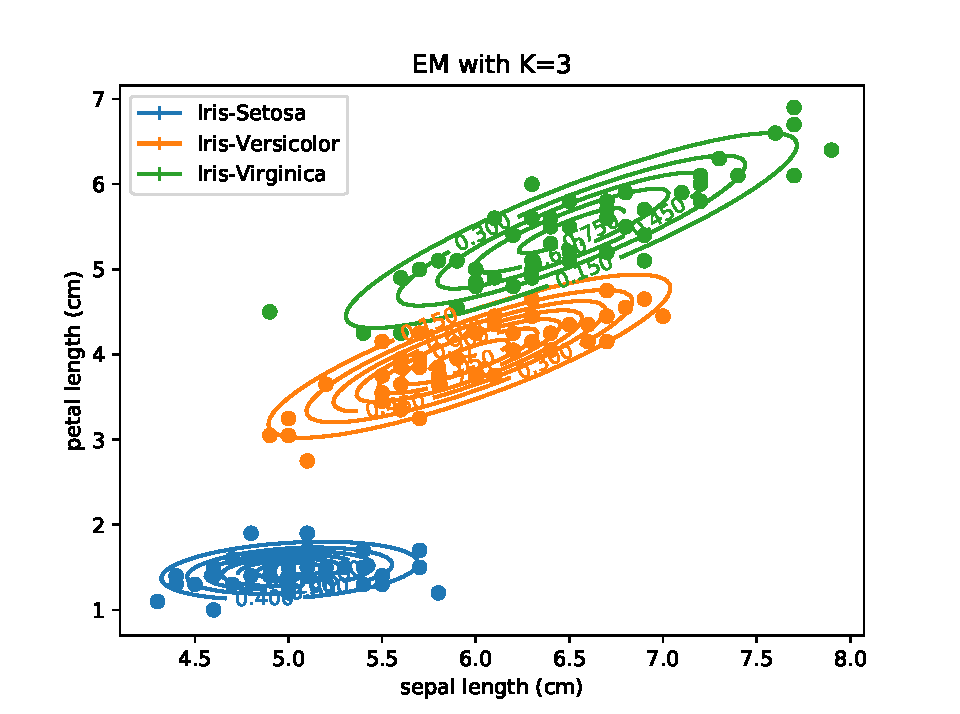
\includegraphics[width=\textwidth]{./Figures/2_1_EM_cont_K3}
	%\caption{$K=3$}
	\end{subfigure}
	\begin{subfigure}{0.6\textwidth}
	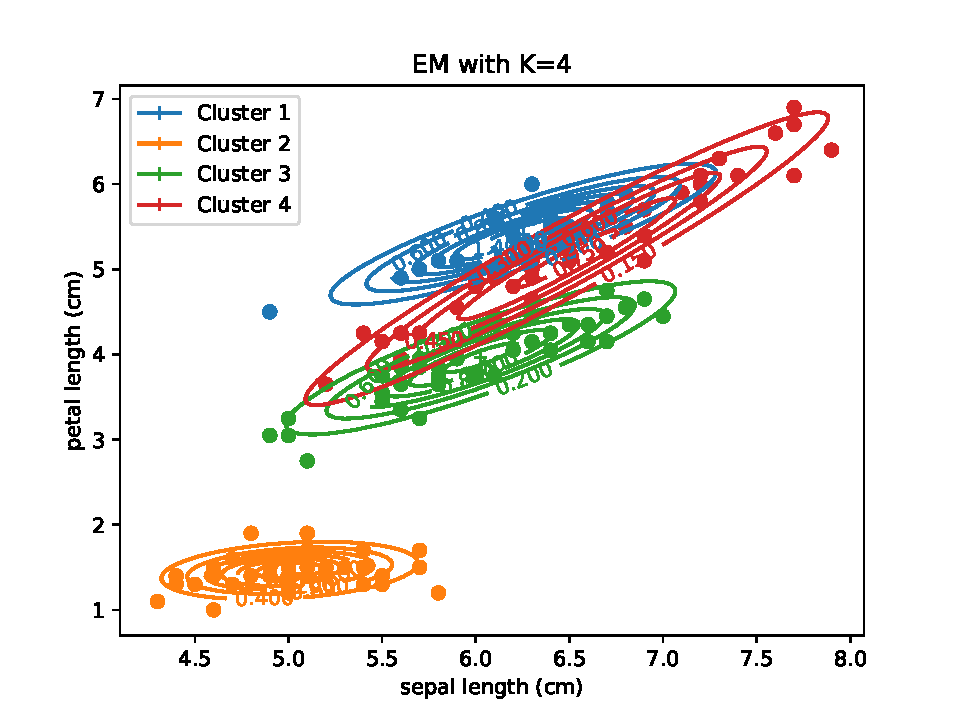
\includegraphics[width=\textwidth]{./Figures/2_1_EM_cont_K4}
	%\caption{$K=4$}
	\end{subfigure}
	}	
	\caption{Results of EM classification with $K=2\dots4$ components.}
	\label{2_1_EM_cont}
\end{figure}

Figure \ref{2_1_EM_cont} shows the dataset and classification results with contours of the used Gaussian kernels for $K=2,3$ and $4$ components. The \textit{Setosa}-Cluster is fully identified with all numbers of components. Using only two components \textit{Versicolor} and \textit{Virginica} are combined into a second cluster. With $K=3$ both remaining classes are classified quite well with only \textit{Versicolor}-samples being misclassified as \textit{Virginica} within the class overlap-region. Using four components a third cluster is formed in this region, leading to incorrect classification. The best results are achieved when using the same number of clusters as the number of classes.

\begin{figure}[!ht]
	\makebox[\textwidth]{
	\begin{subfigure}{0.6\textwidth}
	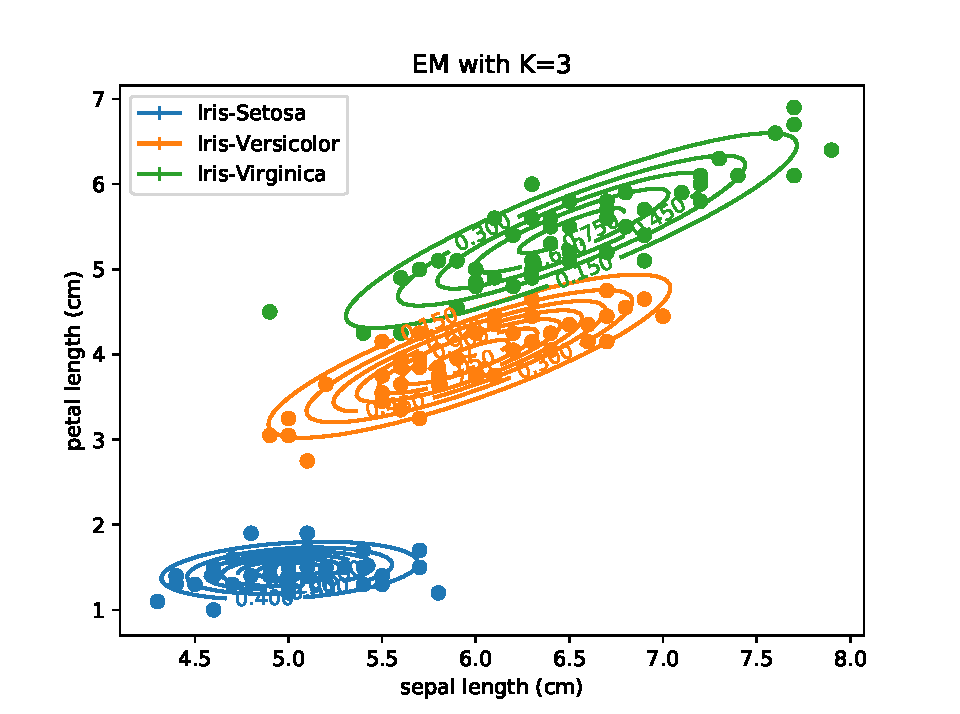
\includegraphics[width=\textwidth]{./Figures/2_1_EM_cont_K3}
	%\caption{Dataset}
	\end{subfigure}
	\begin{subfigure}{0.6\textwidth}
	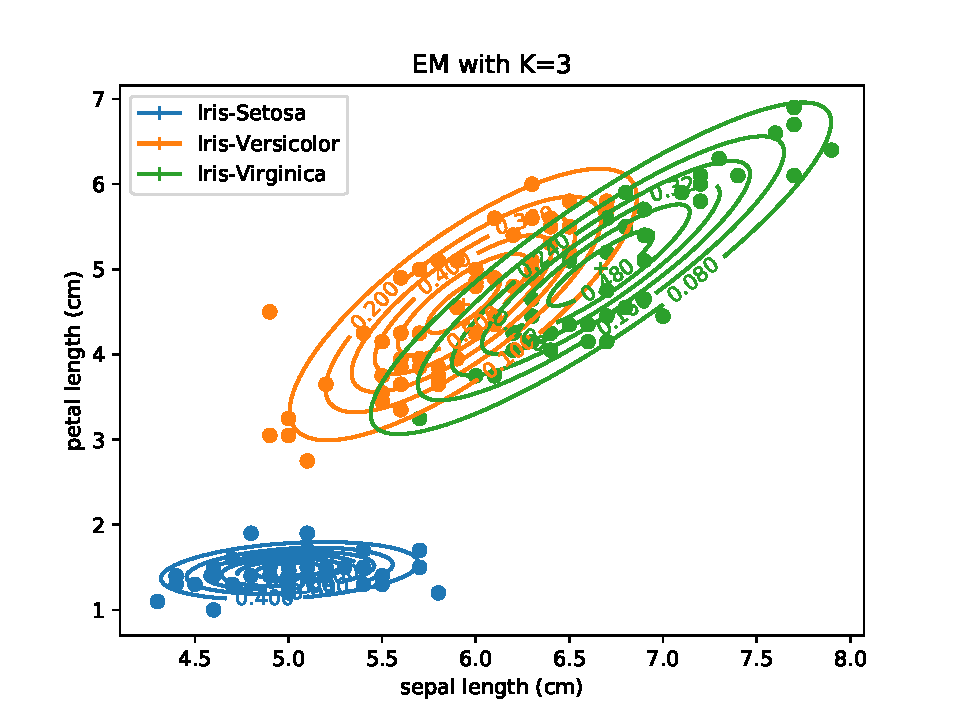
\includegraphics[width=\textwidth]{./Figures/2_1_EM_randinit1}
	%\caption{$K=2$}
	\end{subfigure}
	}
	\makebox[\textwidth]{
	\begin{subfigure}{0.6\textwidth}
	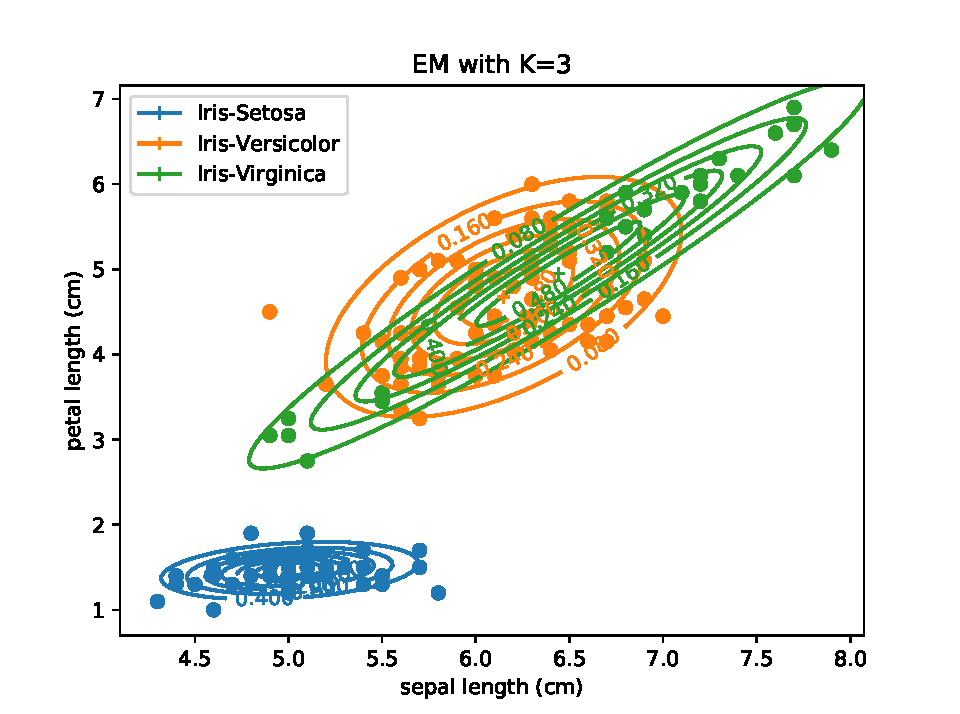
\includegraphics[width=\textwidth]{./Figures/2_1_EM_randinit2}
	%\caption{$K=3$}
	\end{subfigure}
	\begin{subfigure}{0.6\textwidth}
	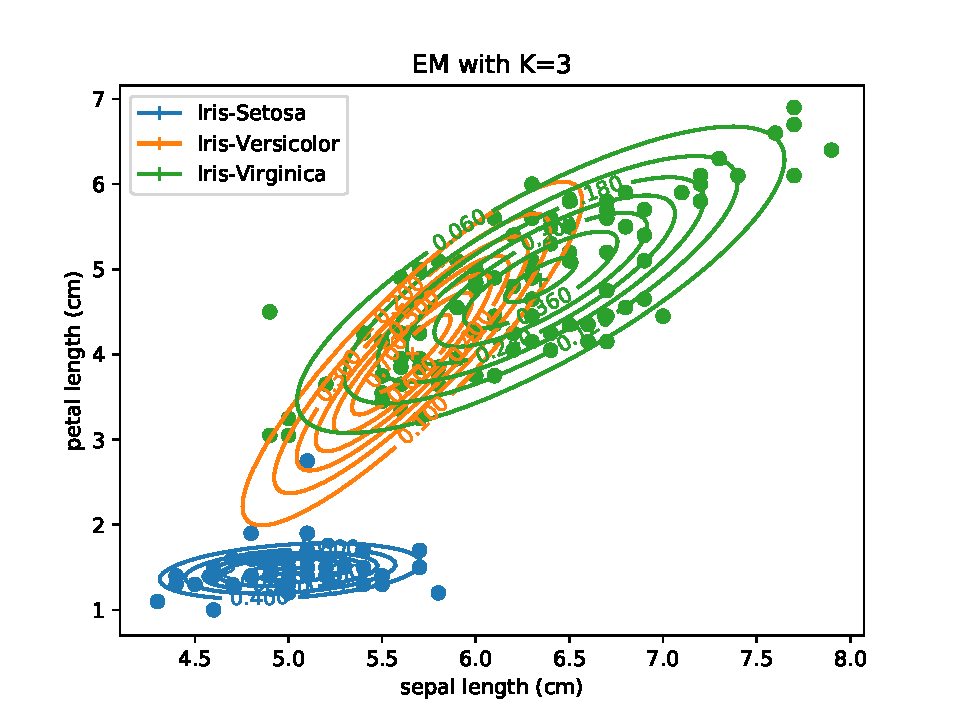
\includegraphics[width=\textwidth]{./Figures/2_1_EM_randinit3}
	%\caption{$K=4$}
	\end{subfigure}
	}	
	\caption{Results of EM classification for several random \texttt{mean0} starting samples.}
	\label{2_1_EM_randinit}
\end{figure}

\newpage

The parameters $\mathbf{\Theta}_0$ are initialised as specified in the lecture notes for all $K$ clusters: \texttt{alpha0} as $1/K$, \texttt{mean0} as random sample of the dataset (different for each cluster), and \texttt{cov0} as the multivariate covariance of the dataset. Because of the non-convex form of the likelihood as a function of $\mathbf{\Theta}_0$, finding the global maximum depends on the starting point of the optimisation process. With some initialisation values one might only find local maxima instead, even though the log-likelihood function increases monotonically over the iterations (s. figure \ref{2_1_EM_likelihood}). Thus the quality of the classification varies greatly for different \texttt{mean0} starting samples (s. figure \ref{2_1_EM_randinit} for some examples). In some instances one of the cluster weights \texttt{alpha} is even set to zero during the optimisation, resulting in only two classes being recognised.\\

\begin{figure}[!ht]
\centering
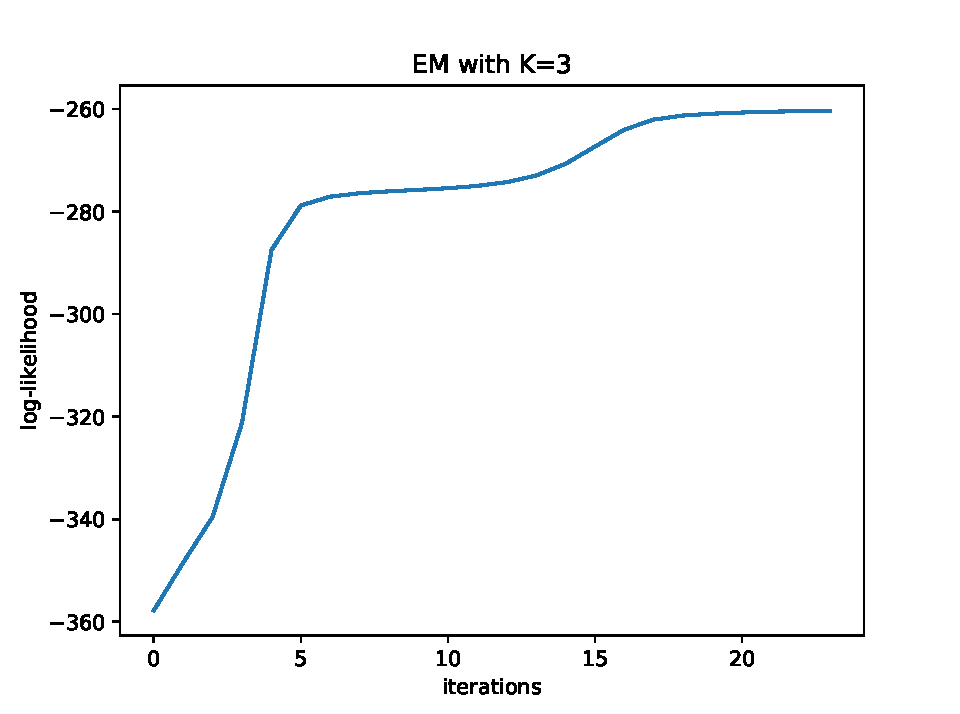
\includegraphics[width=0.6\textwidth]{./Figures/2_1_EM_likelihood_K3}
\caption{Log-likelihood function over iterations for $K=3$ components.}
\label{2_1_EM_likelihood}
\end{figure}

\begin{figure}[!ht]
	\makebox[\textwidth]{
	\begin{subfigure}{0.6\textwidth}
	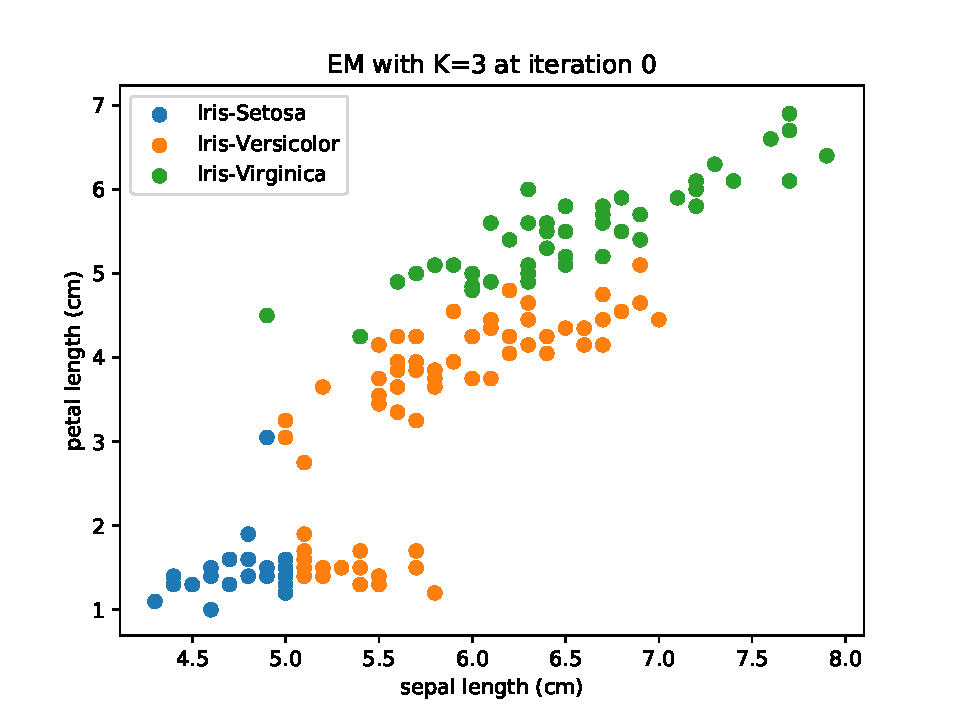
\includegraphics[width=\textwidth]{./Figures/2_1_EM_iter0}
	%\caption{Dataset}
	\end{subfigure}
	\begin{subfigure}{0.6\textwidth}
	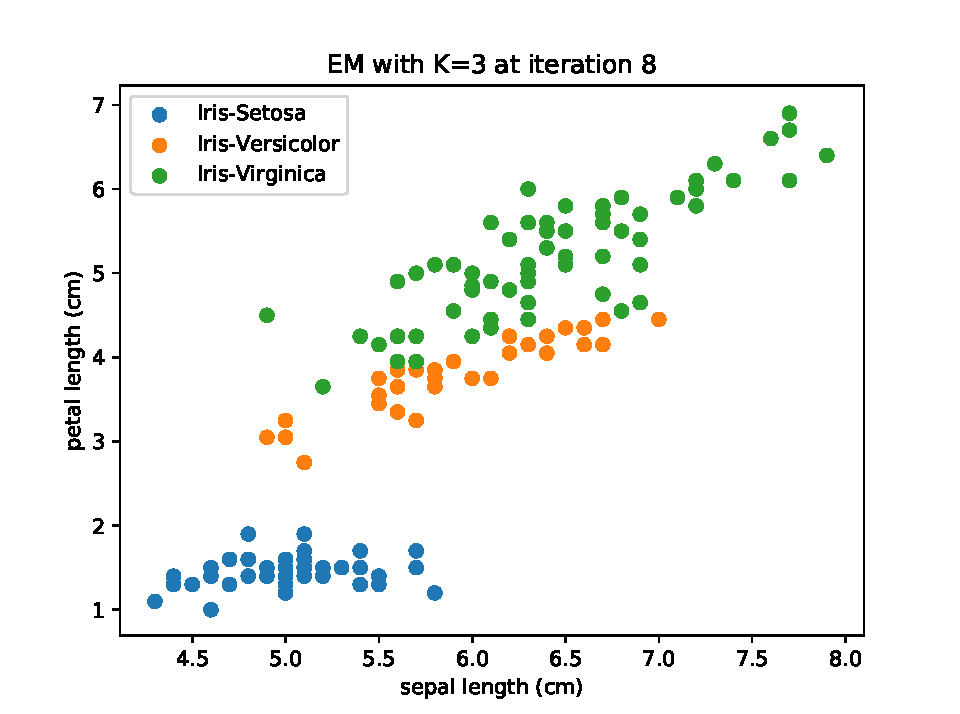
\includegraphics[width=\textwidth]{./Figures/2_1_EM_iter8}
	%\caption{$K=2$}
	\end{subfigure}
	}
	\makebox[\textwidth]{
	\begin{subfigure}{0.6\textwidth}
	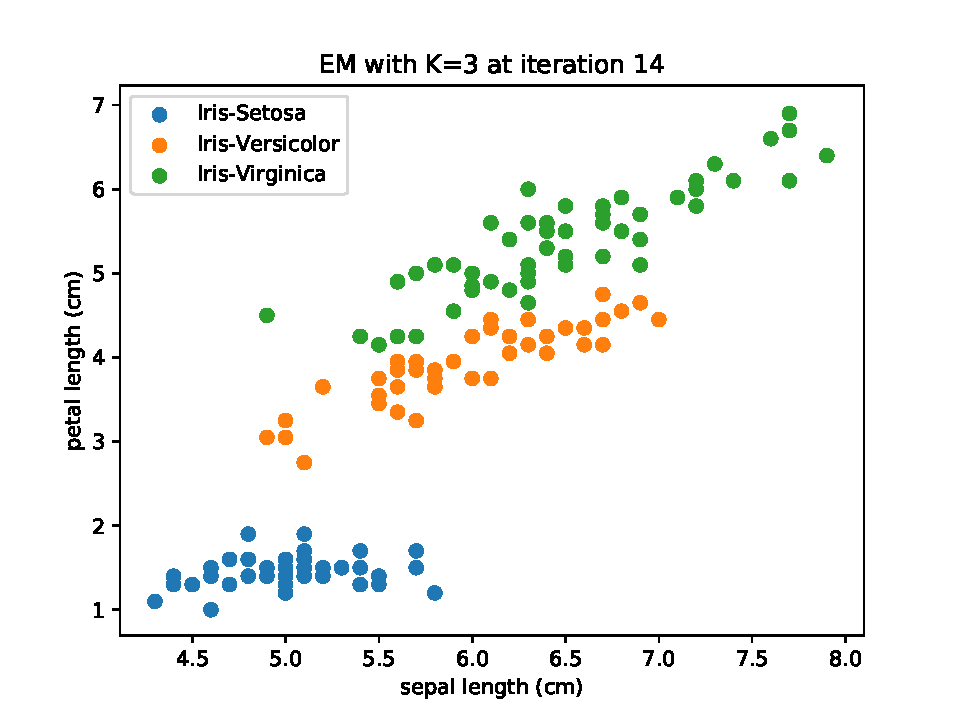
\includegraphics[width=\textwidth]{./Figures/2_1_EM_iter14}
	%\caption{$K=3$}
	\end{subfigure}
	\begin{subfigure}{0.6\textwidth}
	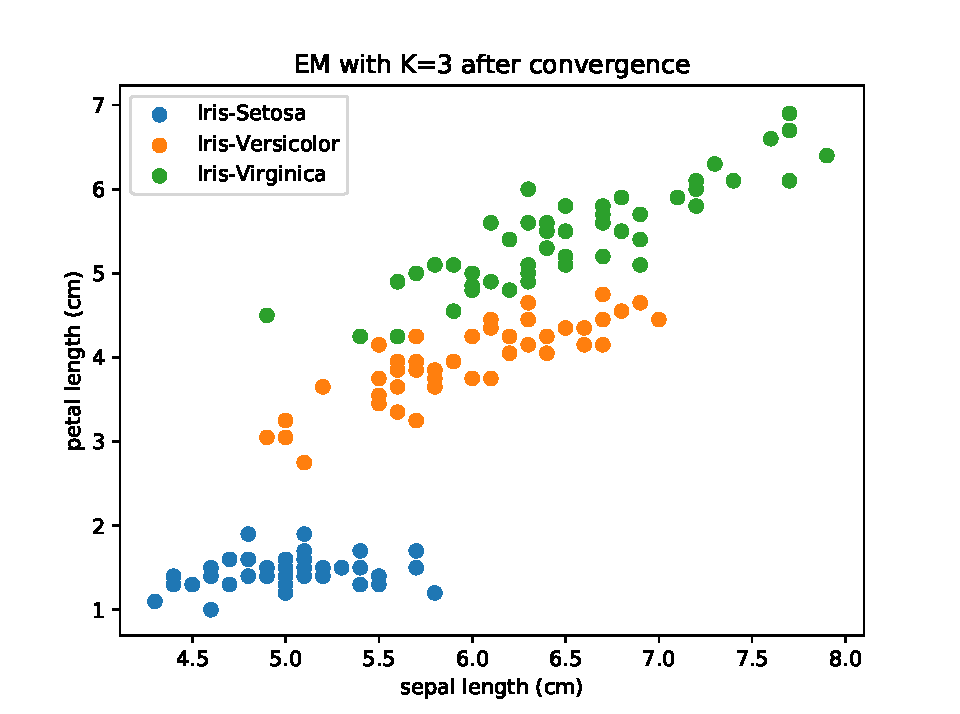
\includegraphics[width=\textwidth]{./Figures/2_1_EM_converged}
	%\caption{$K=4$}
	\end{subfigure}
	}	
	\caption{Results of soft-classification done in E-step.}
	\label{2_1_EM_iter}
\end{figure}

Figure \ref{2_1_EM_iter} shows the results of the soft-classification done in the E-step during the optimisation process. In the beginning the cluster borders (especially between \textit{Setosa} and \textit{Versicolor}) are random, mostly depending on the samples used to initialise \texttt{mean0}. At iteration 8 the \textit{Setosa}-class is correctly classified. In between iteration 8 and the eventual convergence at iteration 23 only the border between \textit{Versicolor}- and \textit{Virginica}-clusters changes slightly. This is, because the log-likelihood (s. figure \ref{2_1_EM_likelihood}) increases only little after the big jump at iterations 3-5.


\clearpage

\subsection{K-means algorithm}

\begin{figure}[!ht]
	\makebox[\textwidth]{
	\begin{subfigure}{0.6\textwidth}
	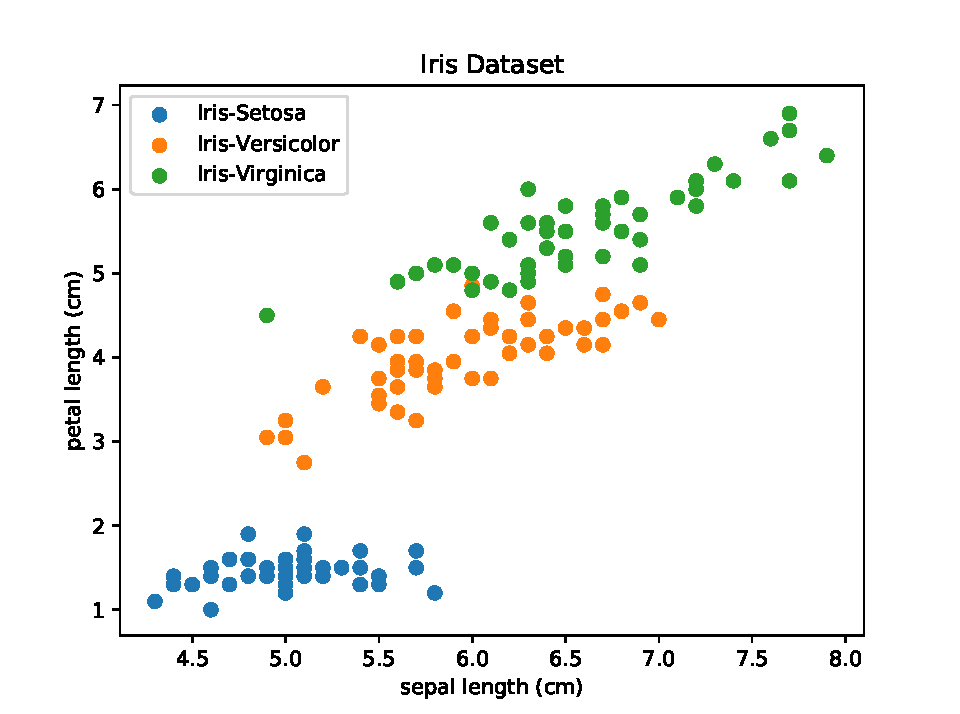
\includegraphics[width=\textwidth]{./Figures/data}
	%\caption{Dataset}
	\end{subfigure}
	\begin{subfigure}{0.6\textwidth}
	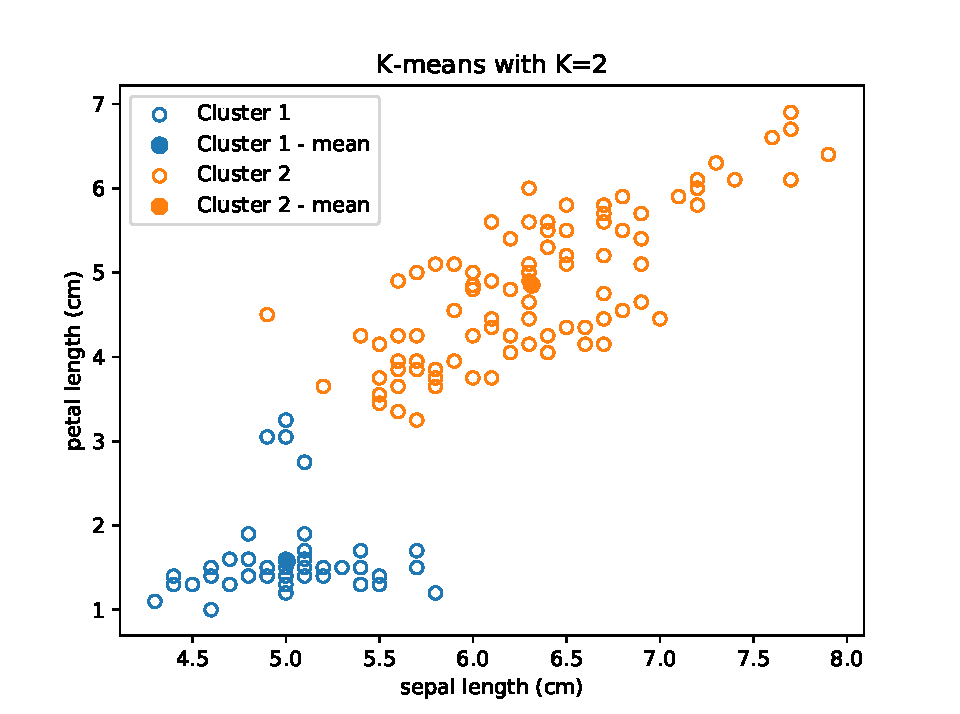
\includegraphics[width=\textwidth]{./Figures/2_1_Kmeans_scatter_K2}
	%\caption{$K=2$}
	\end{subfigure}
	}
	\makebox[\textwidth]{
	\begin{subfigure}{0.6\textwidth}
	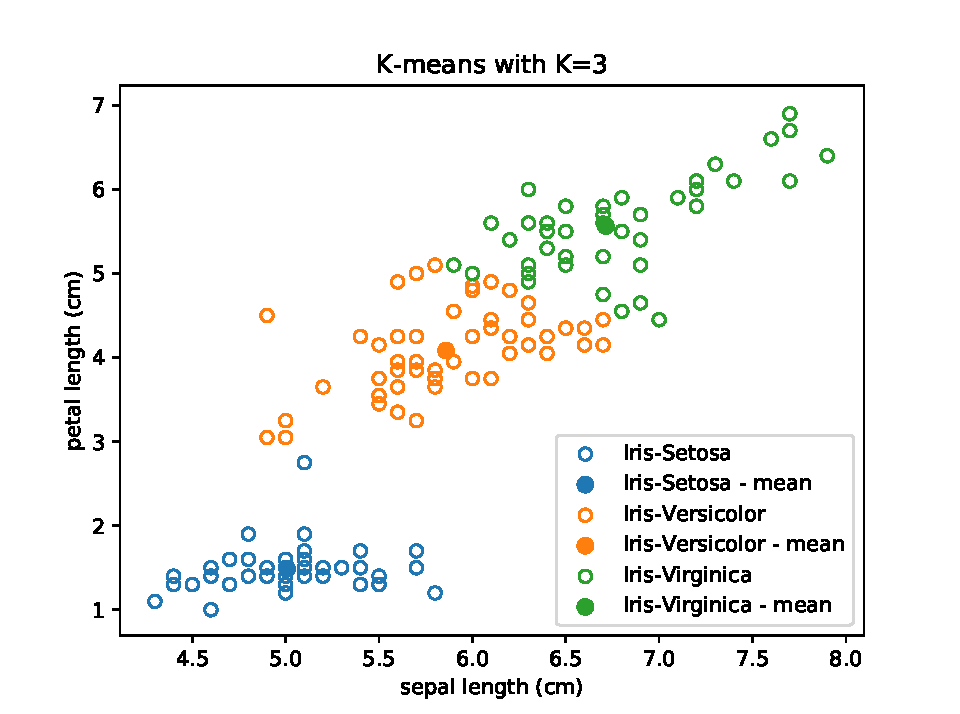
\includegraphics[width=\textwidth]{./Figures/2_1_Kmeans_scatter_K3}
	%\caption{$K=3$}
	\end{subfigure}
	\begin{subfigure}{0.6\textwidth}
	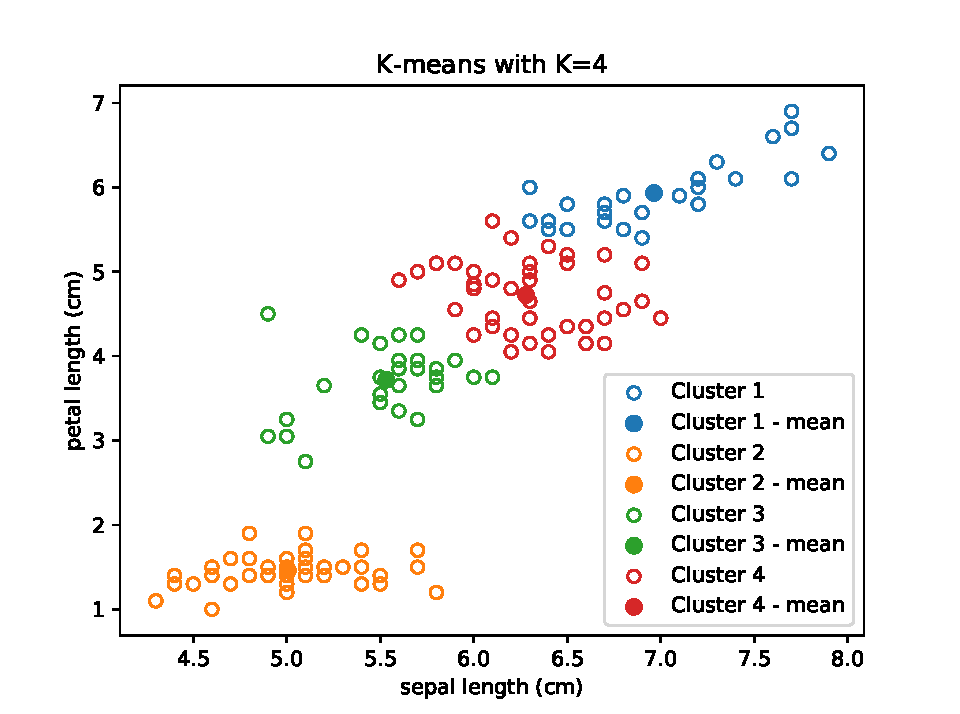
\includegraphics[width=\textwidth]{./Figures/2_1_Kmeans_scatter_K4}
	%\caption{$K=4$}
	\end{subfigure}
	}	
	\caption{Results of K-means classification with $K=2\dots4$ components.}
	\label{2_1_Kmeans_scatter}
\end{figure}

\begin{figure}[!ht]
\centering
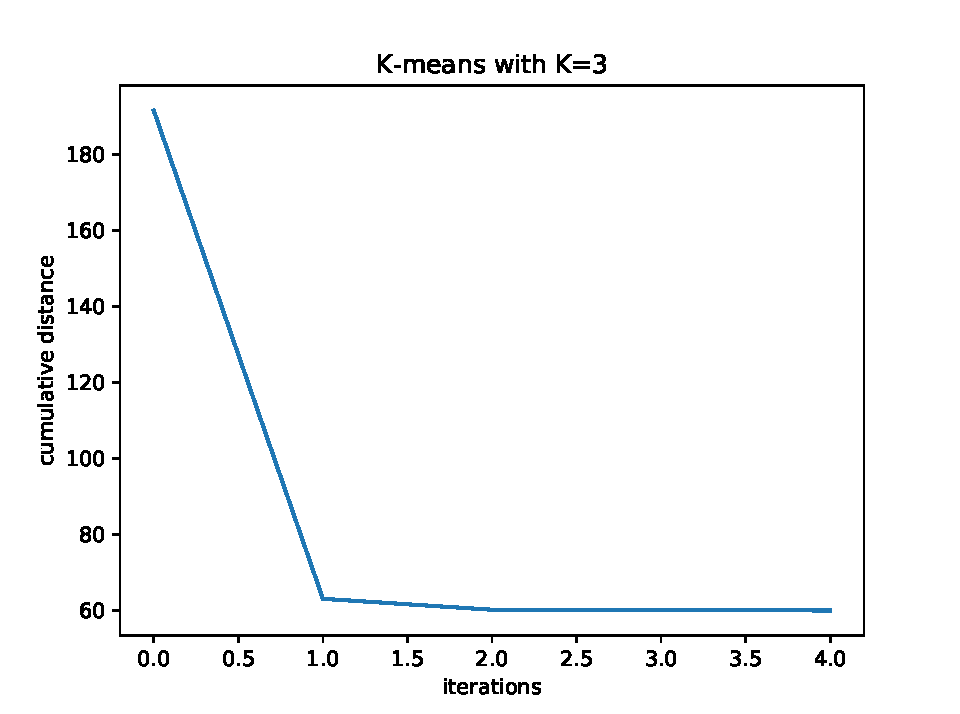
\includegraphics[width=0.6\textwidth]{./Figures/2_1_Kmeans_distance_K3}
\caption{Cumulative distance function over iterations for $K=3$ components.}
\label{2_1_Kmeans_distance}
\end{figure}

\begin{figure}[!ht]
	\makebox[\textwidth]{
	\begin{subfigure}{0.6\textwidth}
	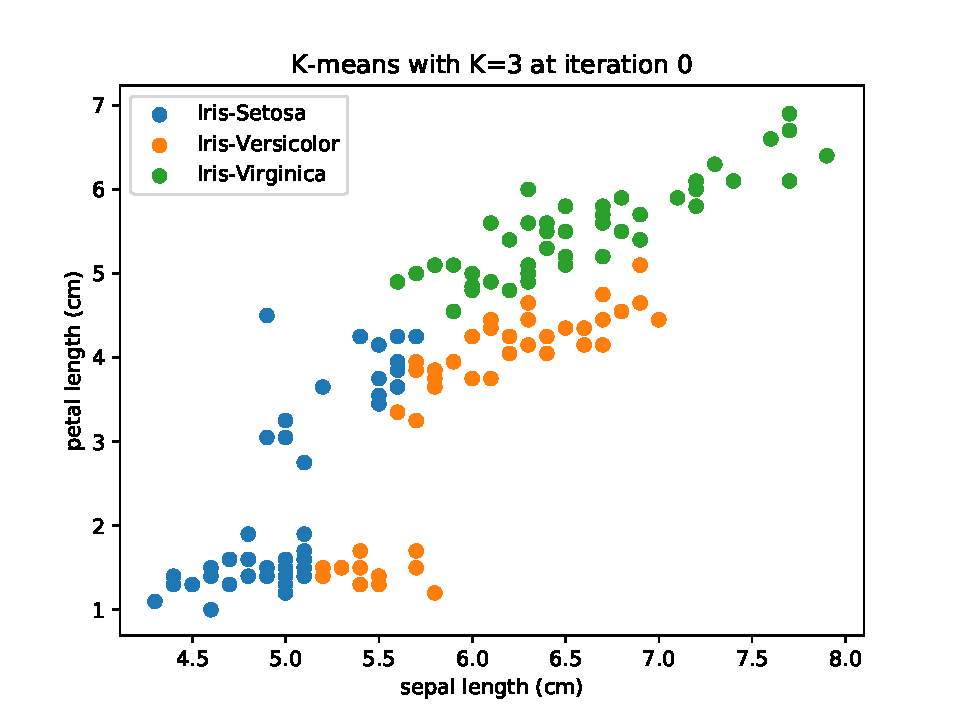
\includegraphics[width=\textwidth]{./Figures/2_1_Kmeans_iter0}
	%\caption{Dataset}
	\end{subfigure}
	\begin{subfigure}{0.6\textwidth}
	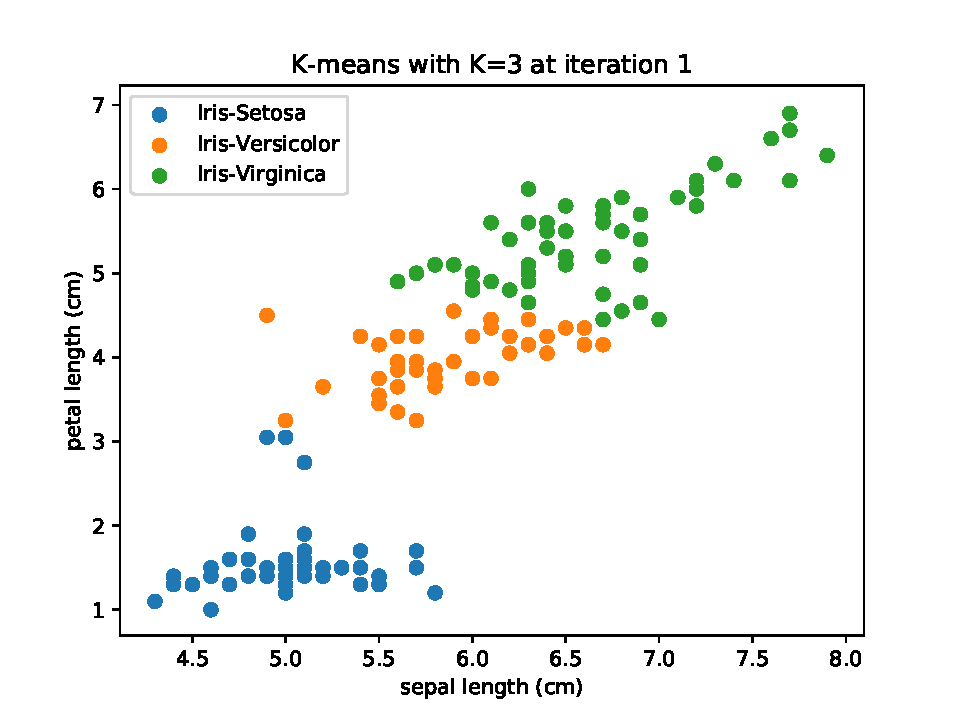
\includegraphics[width=\textwidth]{./Figures/2_1_Kmeans_iter1}
	%\caption{$K=2$}
	\end{subfigure}
	}
	\makebox[\textwidth]{
	\begin{subfigure}{0.6\textwidth}
	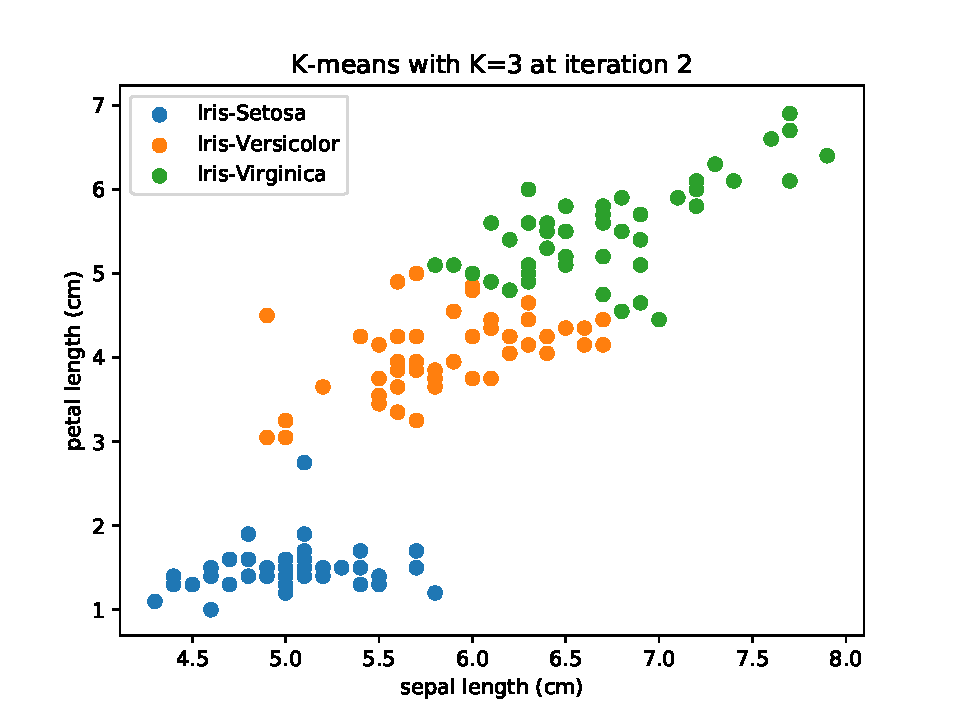
\includegraphics[width=\textwidth]{./Figures/2_1_Kmeans_iter2}
	%\caption{$K=3$}
	\end{subfigure}
	\begin{subfigure}{0.6\textwidth}
	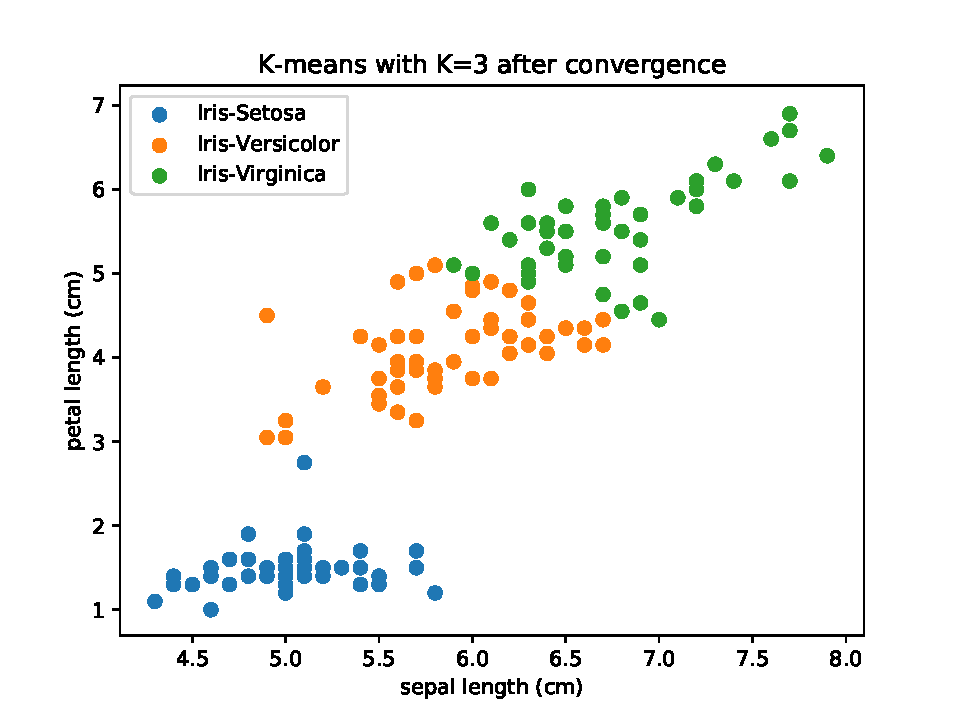
\includegraphics[width=\textwidth]{./Figures/2_1_Kmeans_converged}
	%\caption{$K=4$}
	\end{subfigure}
	}	
	\caption{Results of hard-classification during optimisation.}
	\label{2_1_Kmeans_iter}
\end{figure}


\begin{figure}[!ht]
	\makebox[\textwidth]{
	\begin{subfigure}{0.6\textwidth}
	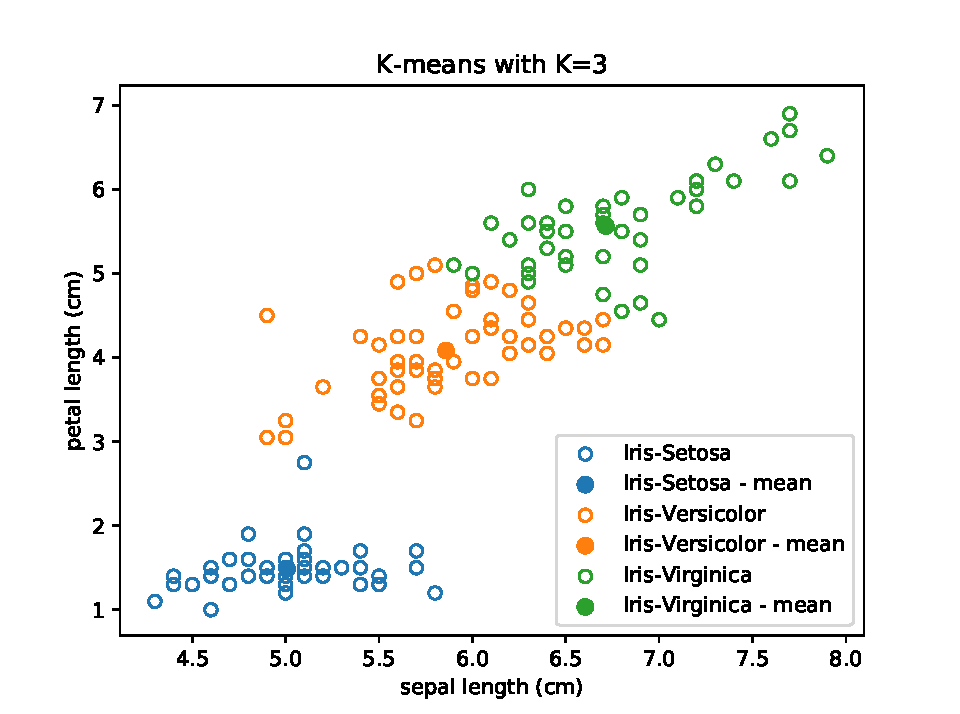
\includegraphics[width=\textwidth]{./Figures/2_1_Kmeans_scatter_K3}
	%\caption{Dataset}
	\end{subfigure}
	\begin{subfigure}{0.6\textwidth}
	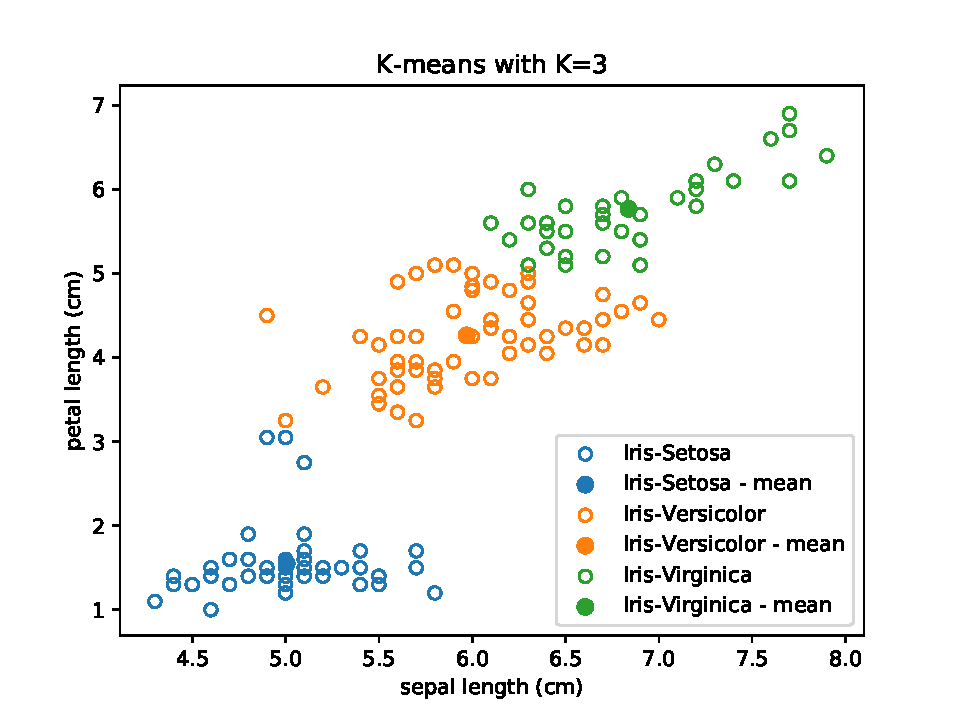
\includegraphics[width=\textwidth]{./Figures/2_1_Kmeans_randinit1}
	%\caption{$K=2$}
	\end{subfigure}
	}
	\makebox[\textwidth]{
	\begin{subfigure}{0.6\textwidth}
	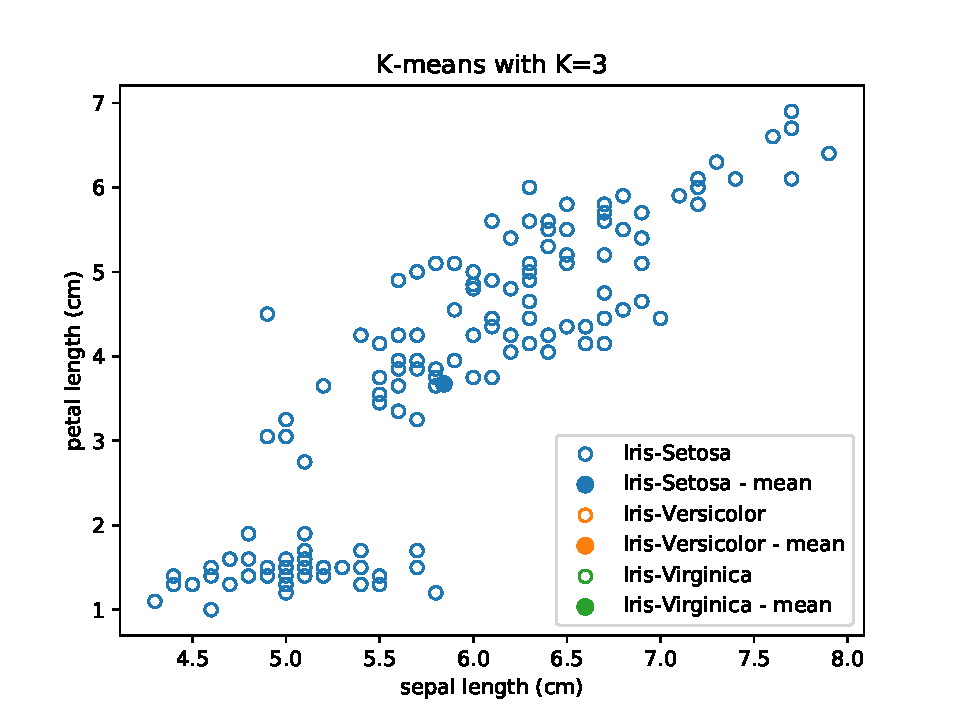
\includegraphics[width=\textwidth]{./Figures/2_1_Kmeans_randinit2}
	%\caption{$K=3$}
	\end{subfigure}
	\begin{subfigure}{0.6\textwidth}
	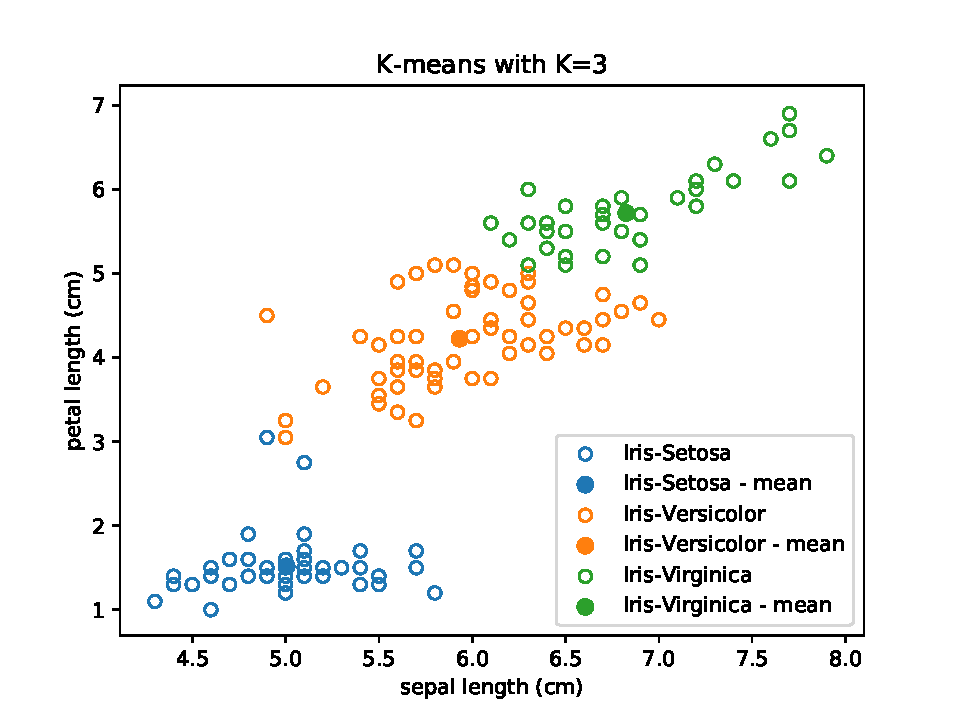
\includegraphics[width=\textwidth]{./Figures/2_1_Kmeans_randinit3}
	%\caption{$K=4$}
	\end{subfigure}
	}	
	\caption{Results of K-means classification for several random \texttt{center0} starting samples.}
	\label{2_1_Kmeans_randinit}
\end{figure}

\clearpage

\section{Classification - 4 dimensional feature}
\subsection{EM algorithm}

\begin{figure}[!ht]
	\makebox[\textwidth]{
	\begin{subfigure}{0.6\textwidth}
	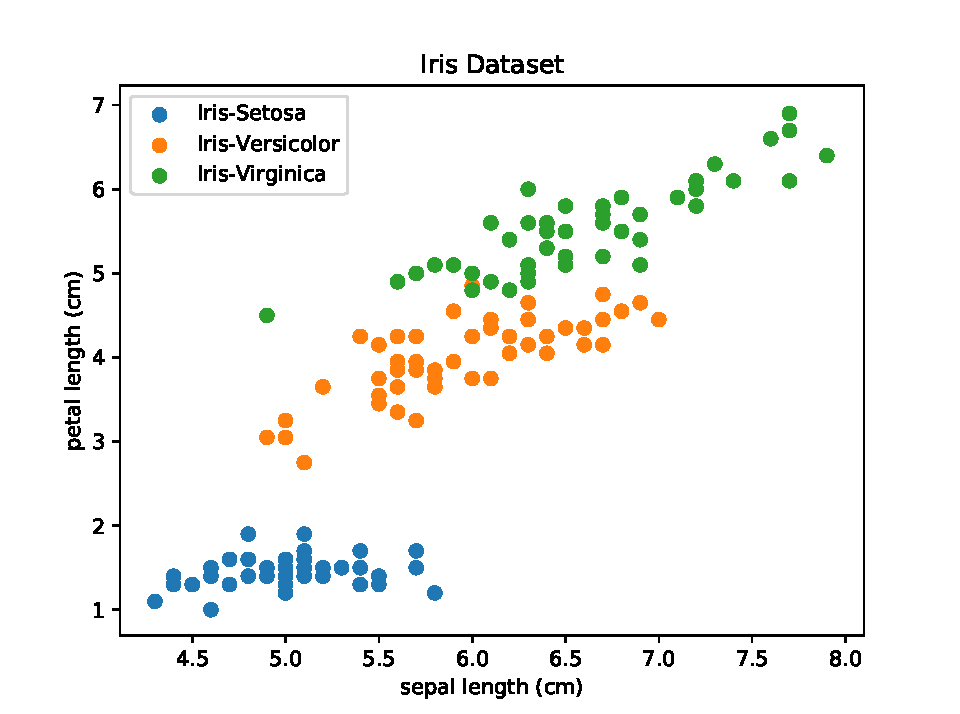
\includegraphics[width=\textwidth]{./Figures/data}
	%\caption{Dataset}
	\end{subfigure}
	\begin{subfigure}{0.6\textwidth}
	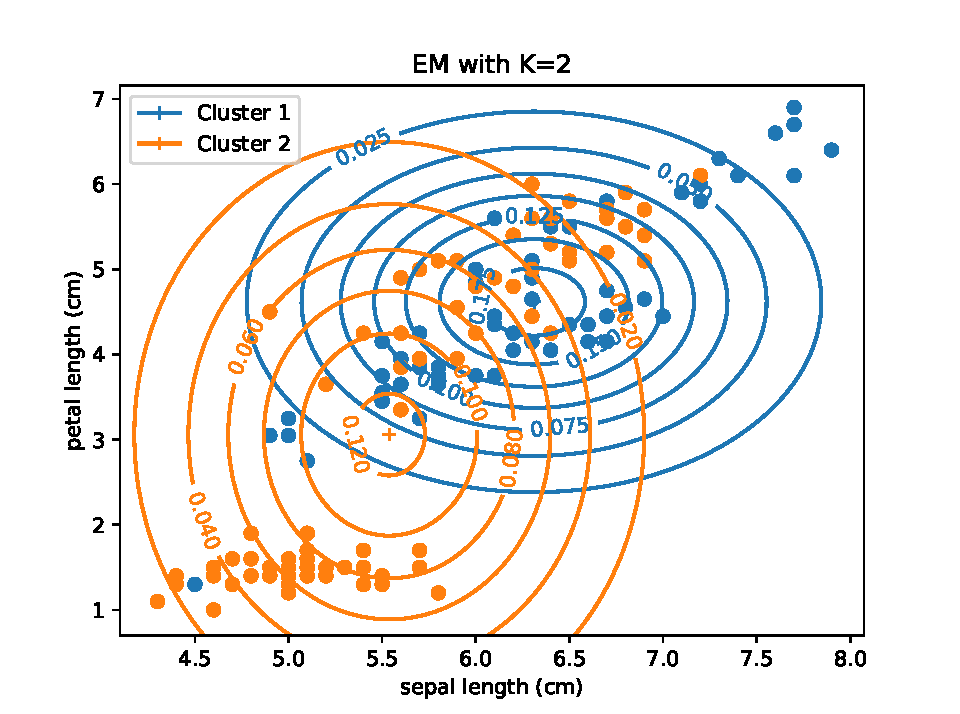
\includegraphics[width=\textwidth]{./Figures/2_2_EM_cont_K2}
	%\caption{$K=2$}
	\end{subfigure}
	}
	\makebox[\textwidth]{
	\begin{subfigure}{0.6\textwidth}
	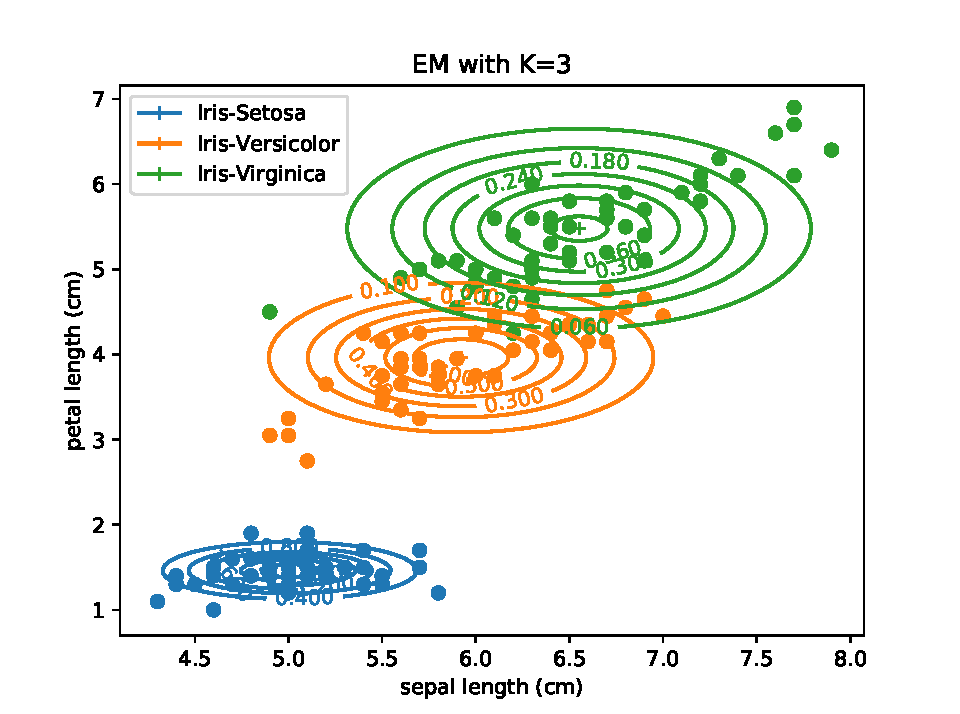
\includegraphics[width=\textwidth]{./Figures/2_2_EM_cont_K3}
	%\caption{$K=3$}
	\end{subfigure}
	\begin{subfigure}{0.6\textwidth}
	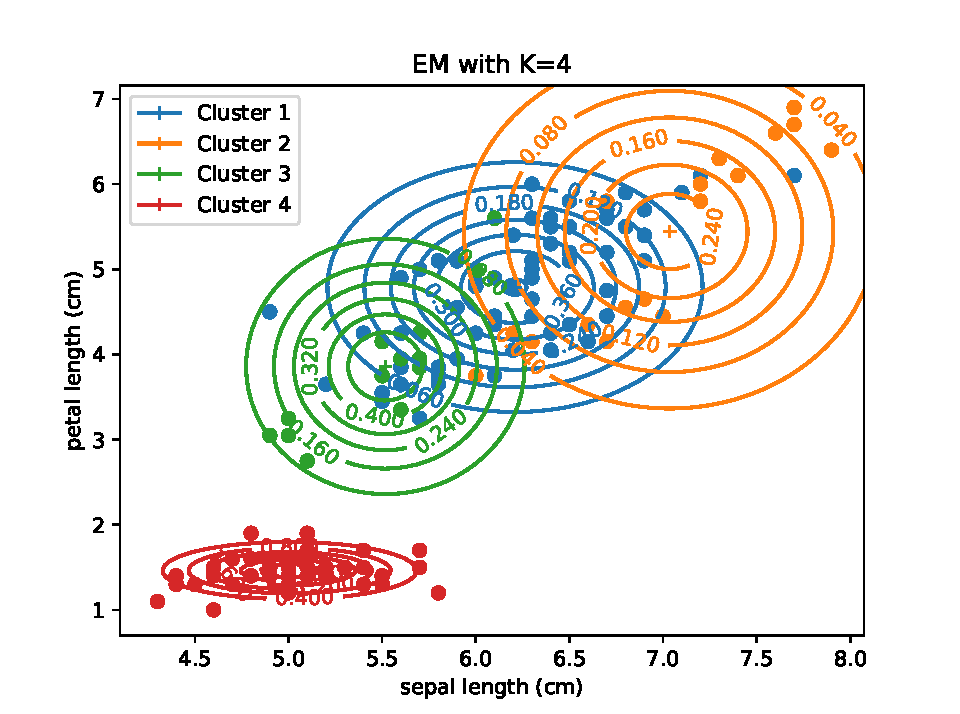
\includegraphics[width=\textwidth]{./Figures/2_2_EM_cont_K4}
	%\caption{$K=4$}
	\end{subfigure}
	}	
	\caption{Results of EM classification with $K=2\dots4$ components.}
	\label{2_2_EM_cont}
\end{figure}

Applying the EM algorithm to the full dataset with $K=3$ components the accuracy after classification stays roughly the same as in scenario 1 (s. figure \ref{2_2_EM_cont}). Using two components the clusters overlap, making it impossible to distinguish any classes. With four components the \textit{Setosa}-class corresponds to Cluster 4, but the remaining clusters overlap as well. The overlap might also occur, because not the whole feature space is plotted. Classes may appear to be better separable when displaying other features.

\begin{figure}[!ht]
	\makebox[\textwidth]{
	\begin{subfigure}{0.6\textwidth}
	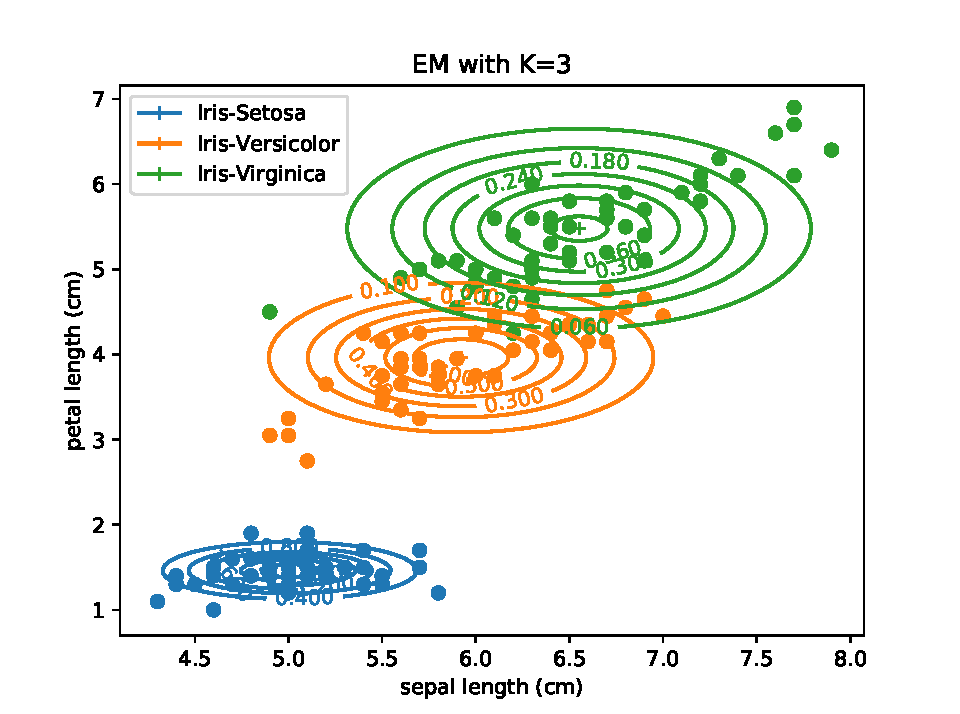
\includegraphics[width=\textwidth]{./Figures/2_2_EM_cont_K3}
	%\caption{Dataset}
	\end{subfigure}
	\begin{subfigure}{0.6\textwidth}
	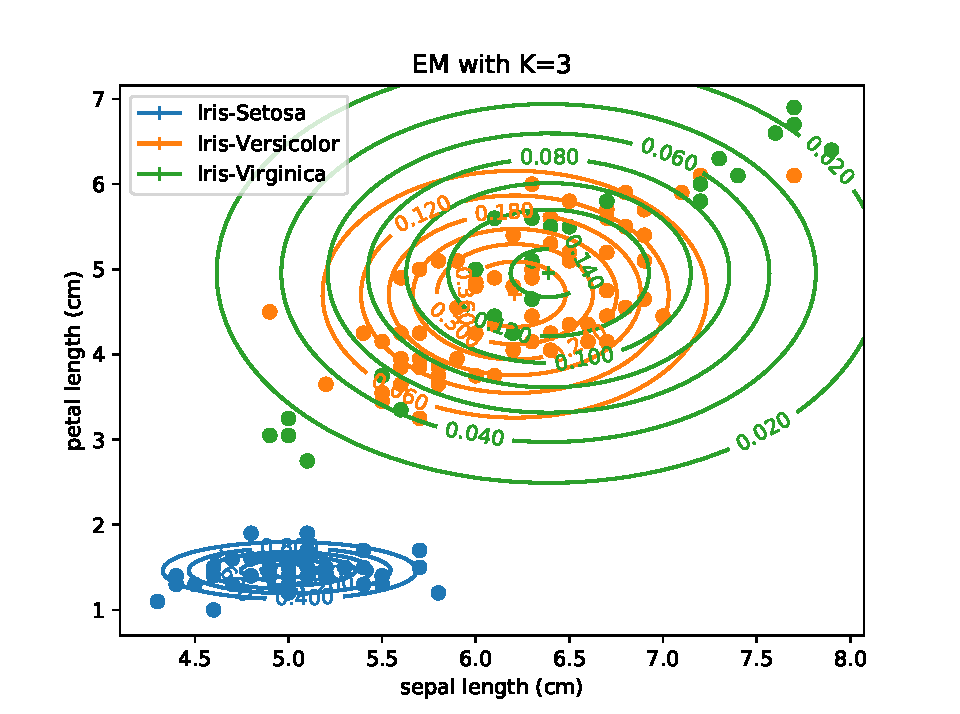
\includegraphics[width=\textwidth]{./Figures/2_2_EM_randinit1}
	%\caption{$K=2$}
	\end{subfigure}
	}
	\makebox[\textwidth]{
	\begin{subfigure}{0.6\textwidth}
	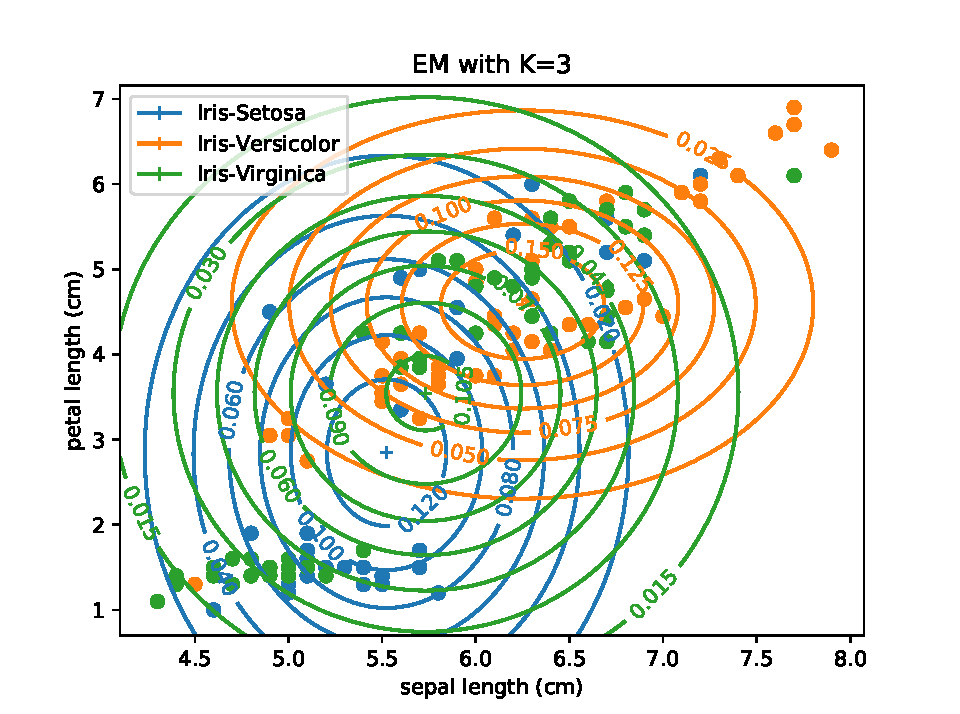
\includegraphics[width=\textwidth]{./Figures/2_2_EM_randinit2}
	%\caption{$K=3$}
	\end{subfigure}
	\begin{subfigure}{0.6\textwidth}
	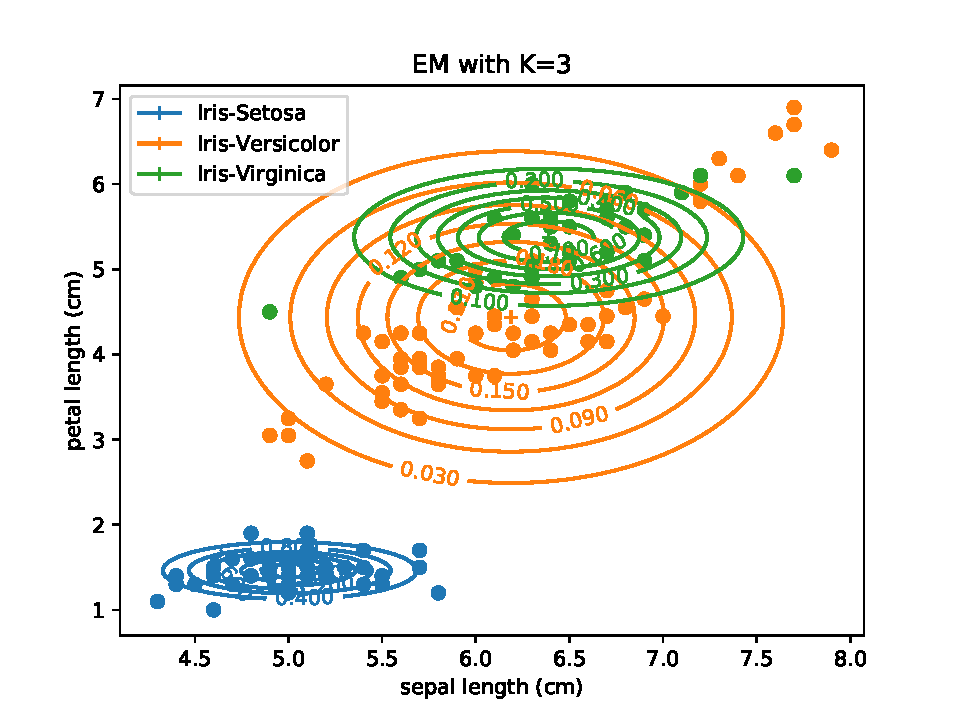
\includegraphics[width=\textwidth]{./Figures/2_2_EM_randinit3}
	%\caption{$K=4$}
	\end{subfigure}
	}	
	\caption{Results of EM classification for several random \texttt{mean0} starting samples.}
	\label{2_2_EM_rand_init}
\end{figure}

Unfortunately the quality of the classification is still strongly dependent on the data samples chosen for \texttt{mean0} (s. figure \ref{2_2_EM_rand_init}).

\begin{figure}[!ht]
\centering
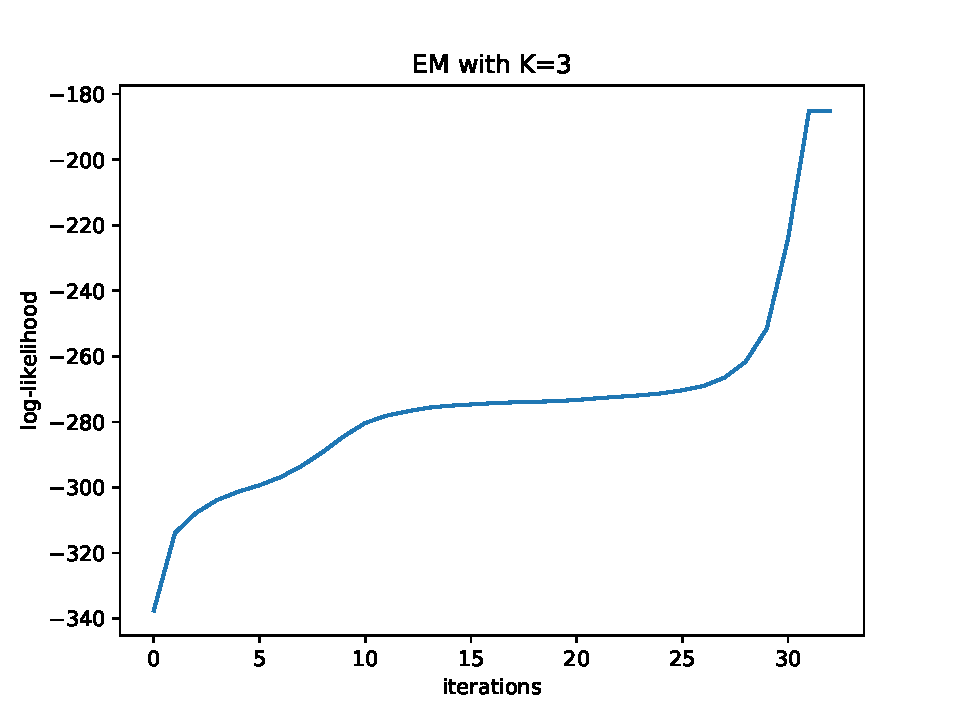
\includegraphics[width=0.6\textwidth]{./Figures/2_2_EM_likelihood_K3}
\caption{Log-likelihood function over iterations for $K=3$ components.}
\label{2_2_EM_likelihood}
\end{figure}

The optimisation process takes longer to converge as with only two features (s. figure \ref{2_2_EM_likelihood}). Because only two features are plotted one cannot comprehend the cluster-formation due to the soft-classification updates in the E-step (s. figure \ref{2_2_EM_iter}) as easily as in scenario 1.

\begin{figure}[!ht]
	\makebox[\textwidth]{
	\begin{subfigure}{0.6\textwidth}
	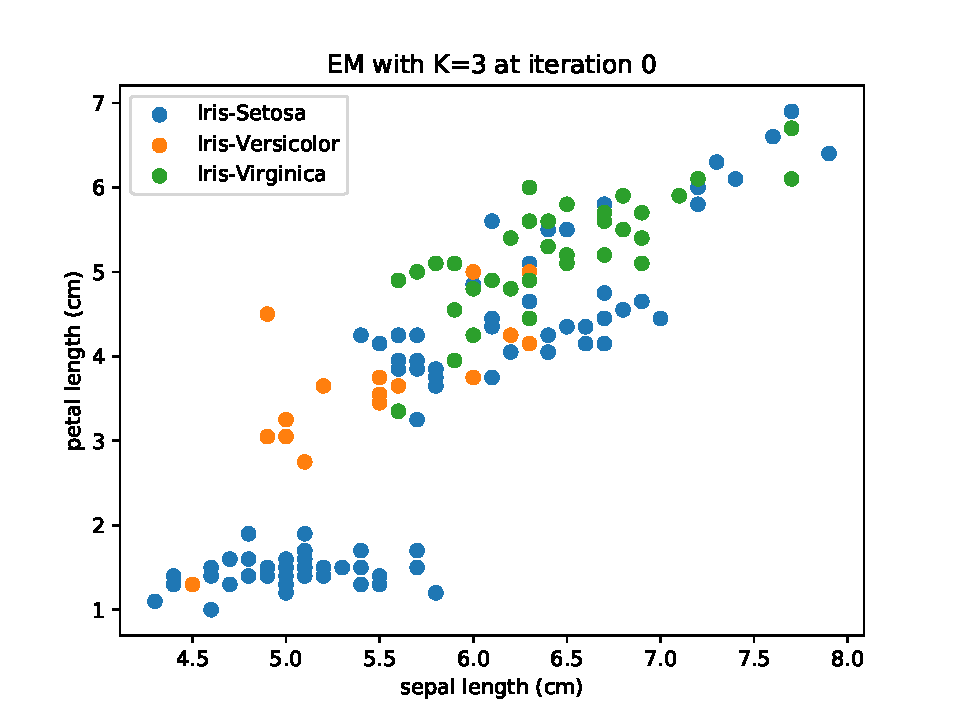
\includegraphics[width=\textwidth]{./Figures/2_2_EM_iter0}
	%\caption{Dataset}
	\end{subfigure}
	\begin{subfigure}{0.6\textwidth}
	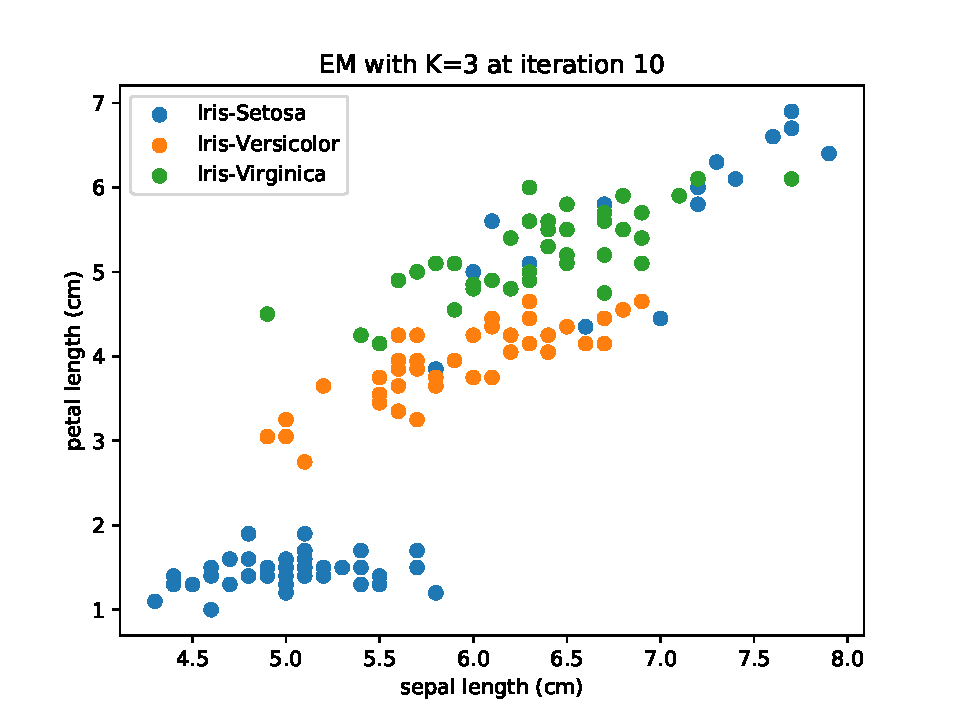
\includegraphics[width=\textwidth]{./Figures/2_2_EM_iter10}
	%\caption{$K=2$}
	\end{subfigure}
	}
	\makebox[\textwidth]{
	\begin{subfigure}{0.6\textwidth}
	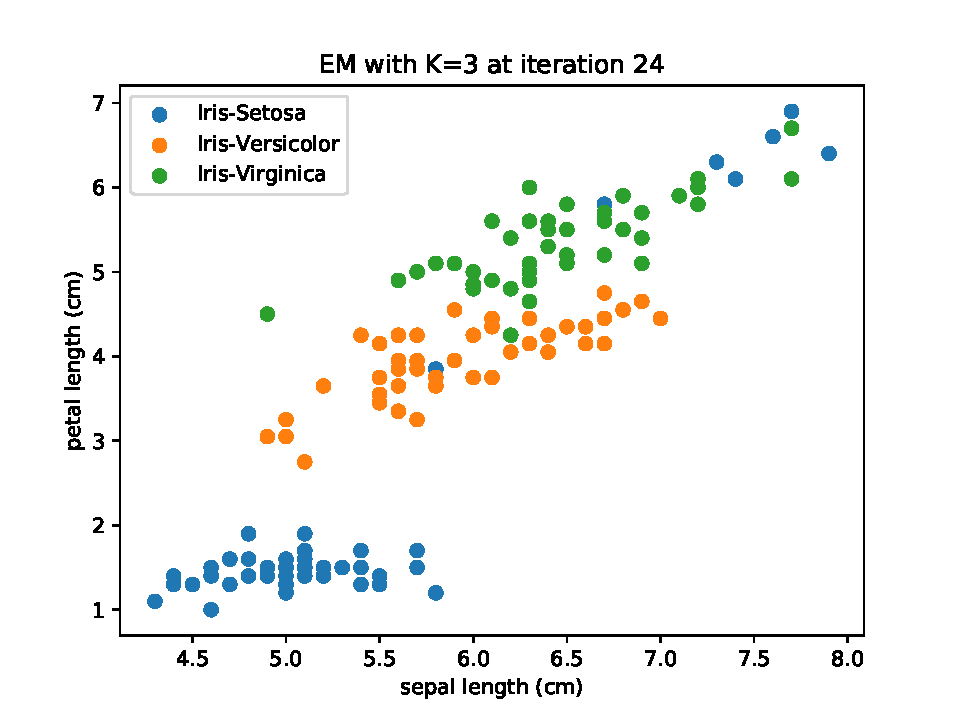
\includegraphics[width=\textwidth]{./Figures/2_2_EM_iter24}
	%\caption{$K=3$}
	\end{subfigure}
	\begin{subfigure}{0.6\textwidth}
	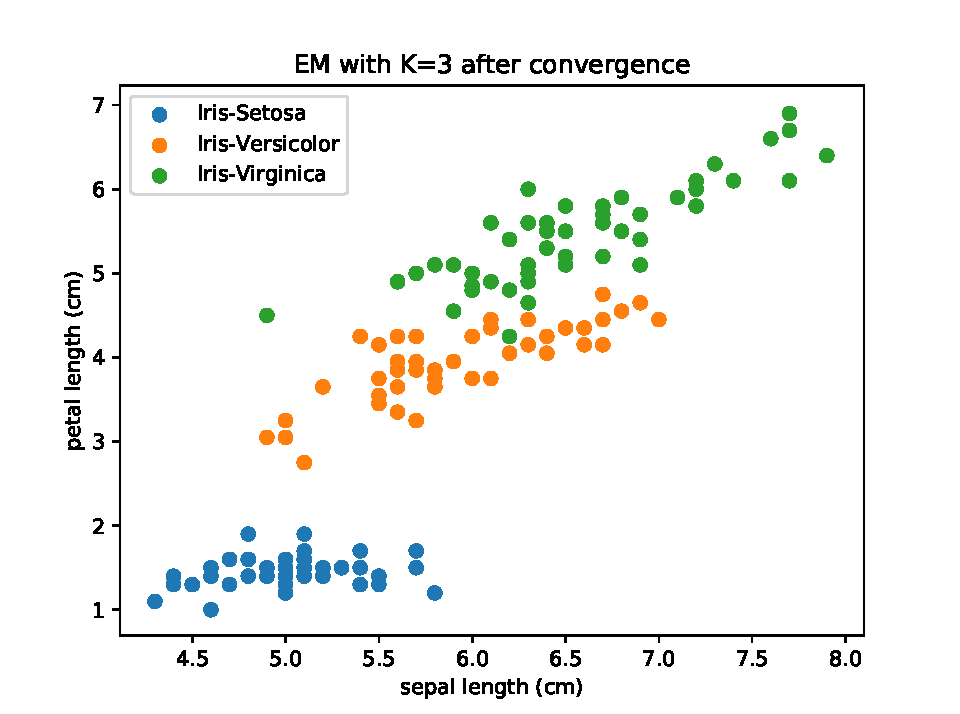
\includegraphics[width=\textwidth]{./Figures/2_2_EM_converged}
	%\caption{$K=4$}
	\end{subfigure}
	}	
	\caption{Results of soft-classification done in E-step.}
	\label{2_2_EM_iter}
\end{figure}

\clearpage

\subsection{EM algorithm with diagonal covariance matrices}

\begin{figure}[!ht]
	\makebox[\textwidth]{
	\begin{subfigure}{0.6\textwidth}
	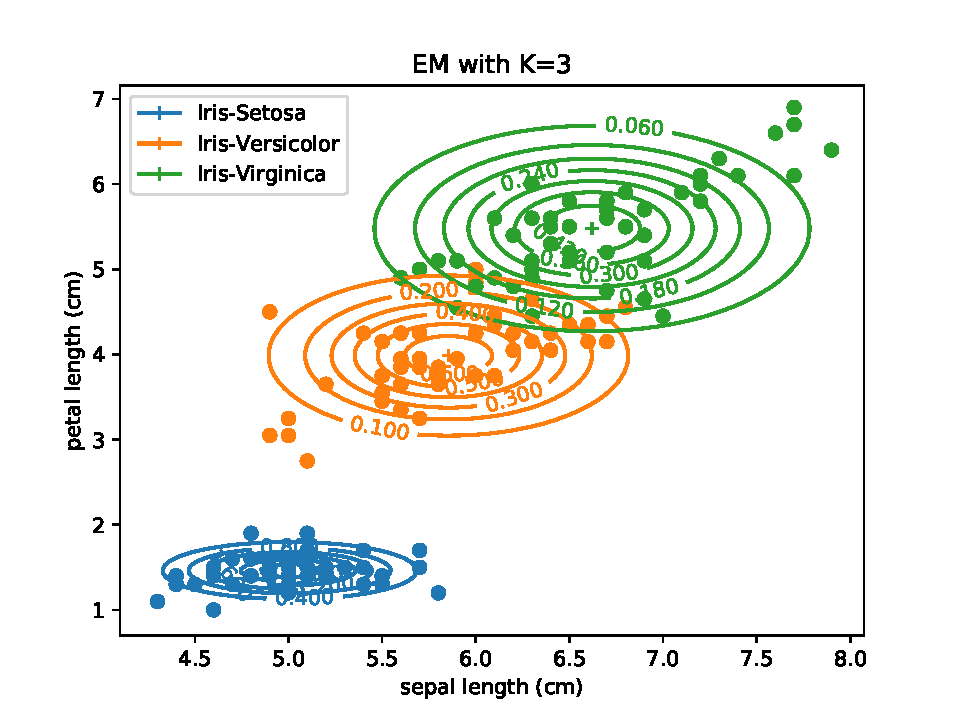
\includegraphics[width=\textwidth]{./Figures/2_2_diagonal_contour_K3}
	\caption{Results of classification}
		\label{2_2_diagonal_cont}
	\end{subfigure}
	\begin{subfigure}{0.6\textwidth}
	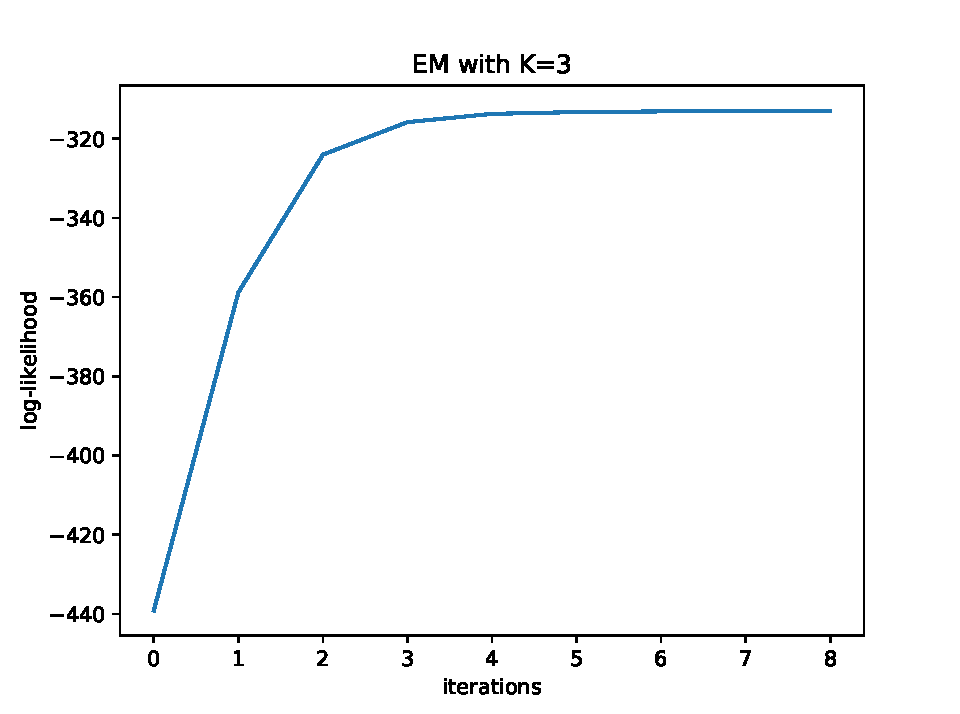
\includegraphics[width=\textwidth]{./Figures/2_2_diagonal_likelihood_K3}
	\caption{Log-likelihood}
		\label{2_2_diagonal_likelihood}
	\end{subfigure}
	}
	\caption{Results of EM classification with diagonal covariance matrices.}
	\label{2_2_diagonal}
\end{figure}

Confining the structure of the covariance matrices to diagonal matrices sets the covariance between the features to zero. This prevents the Gaussian kernels displayed in figure \ref{2_2_diagonal_cont} from being tilted, which corresponds well with the dataset. While the resulting classification is not quite as accurate as with the very best results using non-diagonal covariance matrices (visible in the overlap region of \textit{Versicolor} and \textit{Virginica}), the quality of the results is not dependent on the initialisation of \texttt{mean0} anymore. Because there are fewer degrees of freedom with only diagonal covariance matrices the algorithm also converges much faster (s. figure \ref{2_2_diagonal_likelihood}).

\clearpage

\subsection{K-means algorithm}

\begin{figure}[!ht]
	\makebox[\textwidth]{
	\begin{subfigure}{0.6\textwidth}
	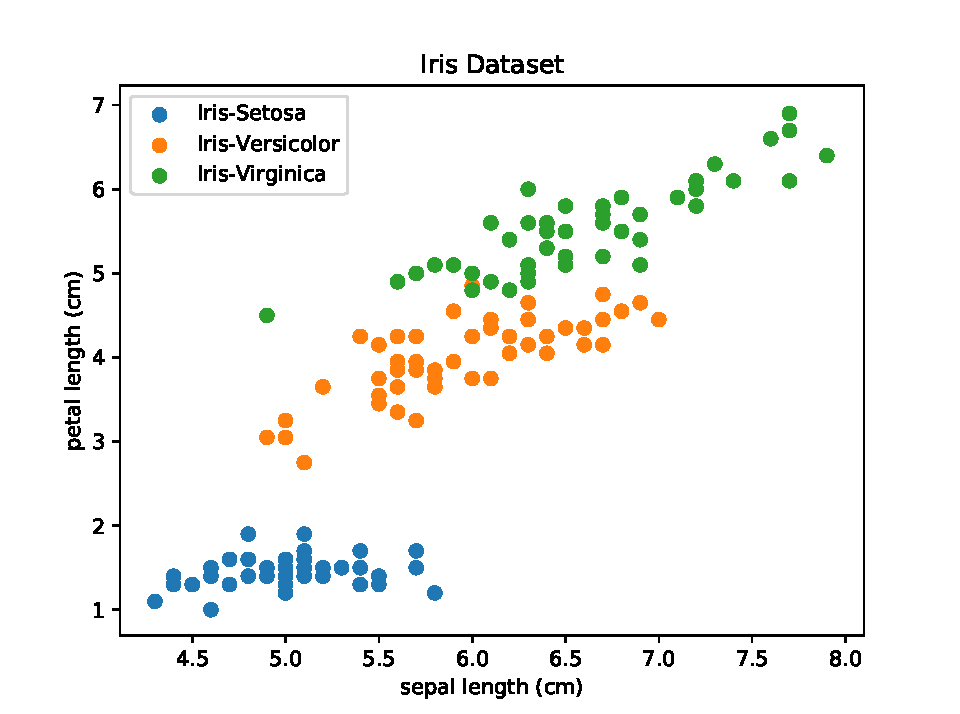
\includegraphics[width=\textwidth]{./Figures/data}
	%\caption{Dataset}
	\end{subfigure}
	\begin{subfigure}{0.6\textwidth}
	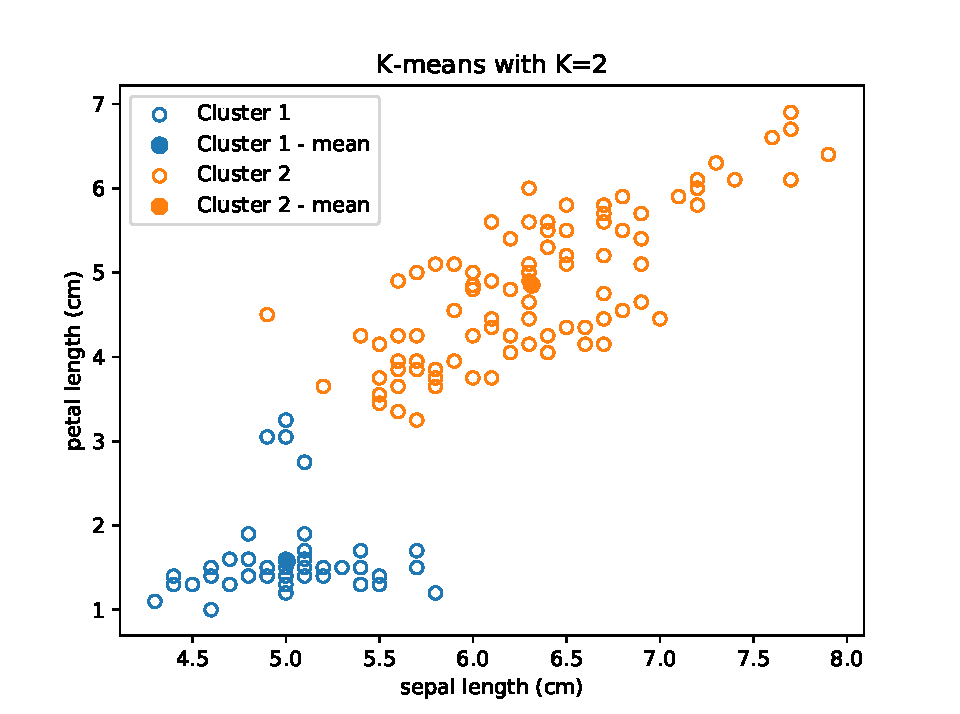
\includegraphics[width=\textwidth]{./Figures/2_2_Kmeans_scatter_K2}
	%\caption{$K=2$}
	\end{subfigure}
	}
	\makebox[\textwidth]{
	\begin{subfigure}{0.6\textwidth}
	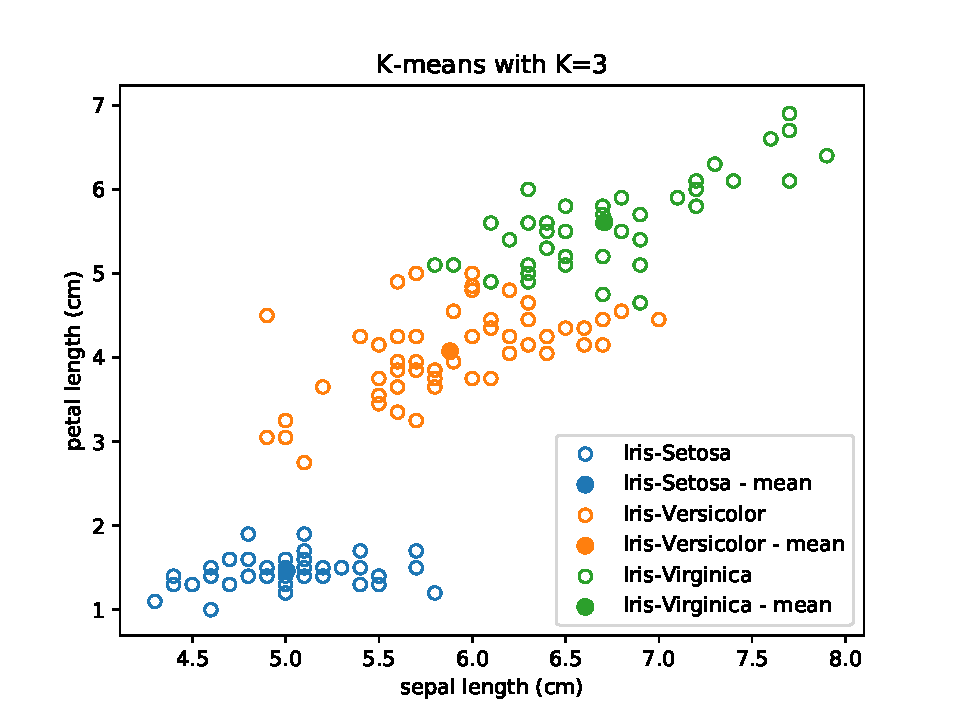
\includegraphics[width=\textwidth]{./Figures/2_2_Kmeans_scatter_K3}
	%\caption{$K=3$}
	\end{subfigure}
	\begin{subfigure}{0.6\textwidth}
	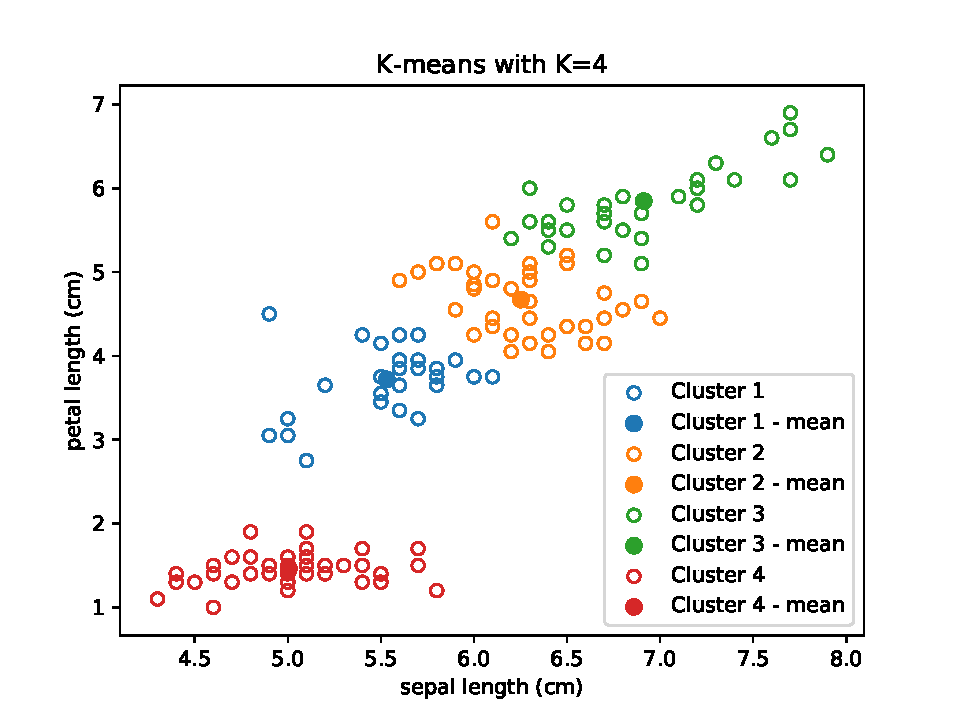
\includegraphics[width=\textwidth]{./Figures/2_2_Kmeans_scatter_K4}
	%\caption{$K=4$}
	\end{subfigure}
	}	
	\caption{Results of K-means classification with $K=2\dots4$ components.}
	\label{2_2_Kmeans_scatter}
\end{figure}

While the classification result with two components using the whole feature set is the same as in scenario 1, the classification using three clusters improves (s. figure \ref{2_2_Kmeans_scatter}). Now \textit{Setosa} is classified correctly and there are fewer misclassified samples on the border between \textit{Versicolor} and \textit{Virginica}. Clustering with four components leads to similar results as in scenario 1 with only a slight shift of the borders between Clusters 2 and 3 (1 and 4 in scenario 1, respectively).

\begin{figure}[!ht]
	\makebox[\textwidth]{
	\begin{subfigure}{0.6\textwidth}
	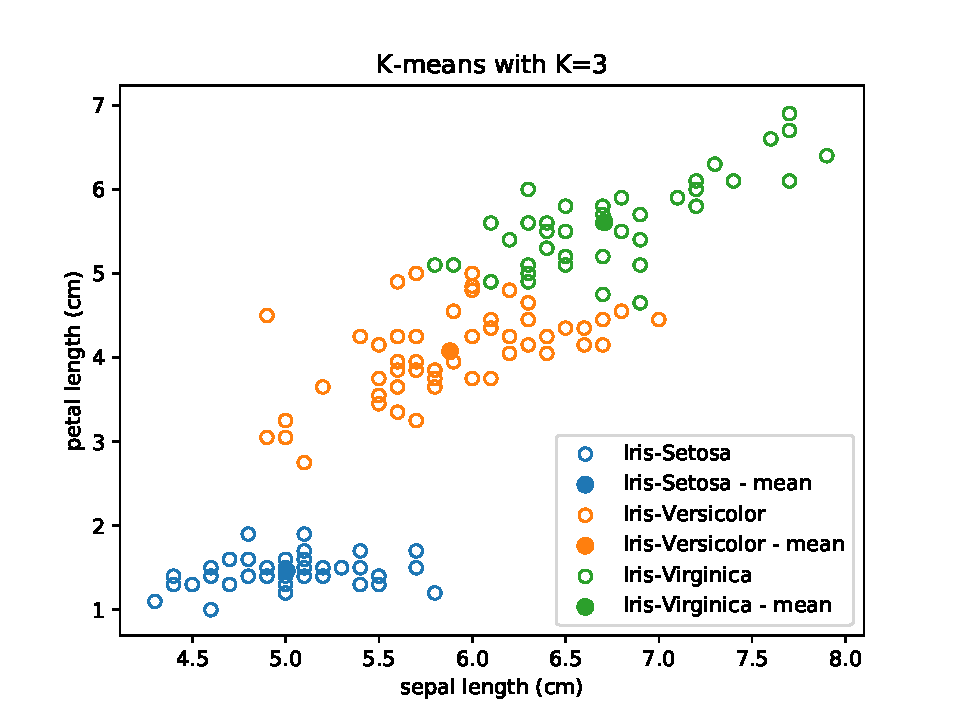
\includegraphics[width=\textwidth]{./Figures/2_2_Kmeans_scatter_K3}
	%\caption{Dataset}
	\end{subfigure}
	\begin{subfigure}{0.6\textwidth}
	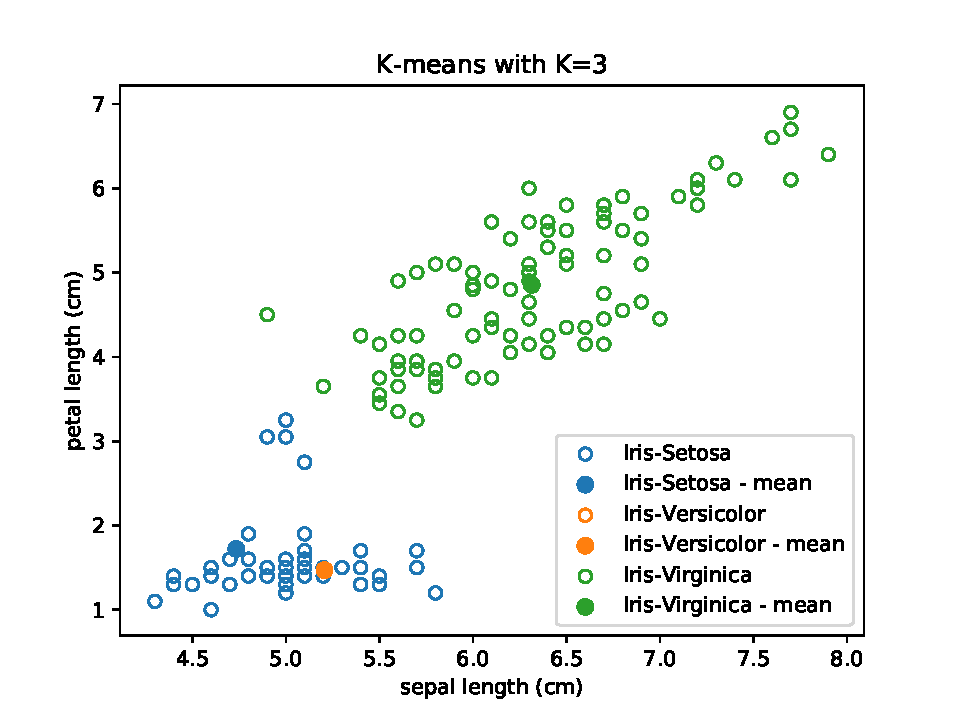
\includegraphics[width=\textwidth]{./Figures/2_2_Kmeans_randinit1}
	%\caption{$K=2$}
	\end{subfigure}
	}
	\makebox[\textwidth]{
	\begin{subfigure}{0.6\textwidth}
	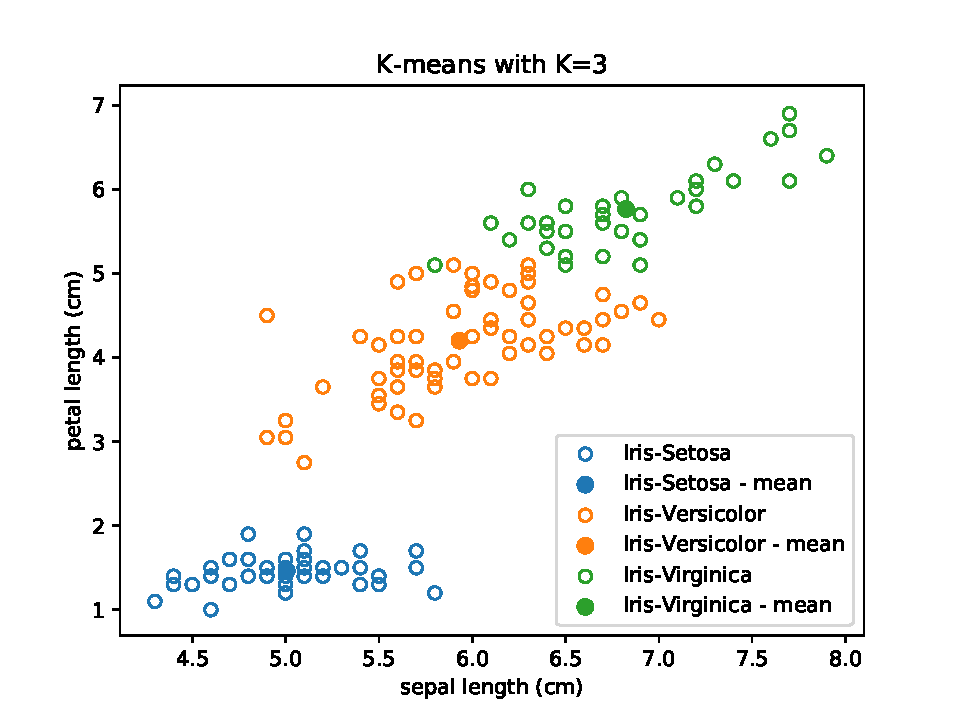
\includegraphics[width=\textwidth]{./Figures/2_2_Kmeans_randinit2}
	%\caption{$K=3$}
	\end{subfigure}
	\begin{subfigure}{0.6\textwidth}
	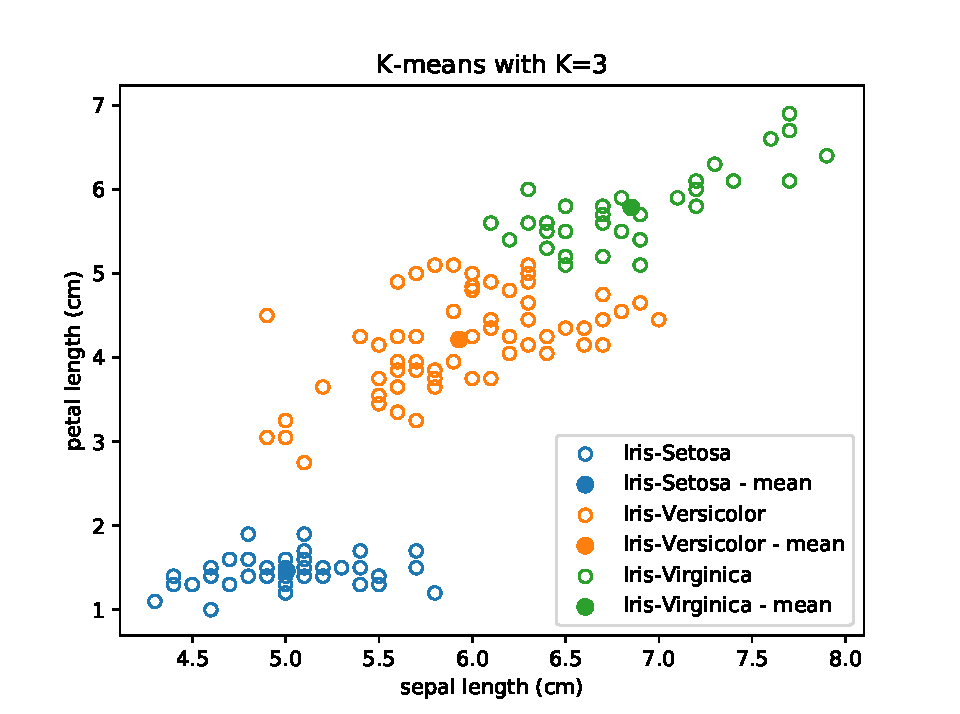
\includegraphics[width=\textwidth]{./Figures/2_2_Kmeans_randinit3}
	%\caption{$K=4$}
	\end{subfigure}
	}	
	\caption{Results of K-means classification for several random \texttt{center0} starting samples.}
	\label{2_2_Kmeans_randinit}
\end{figure}

Except for some instances where there were only two clusters found, the quality of the achieved classification results varies only slightly depending on the initialisation of \texttt{center0} - about the same as in scenario 1 (s. figure \ref{2_2_Kmeans_randinit}).

\begin{figure}[!ht]
\centering
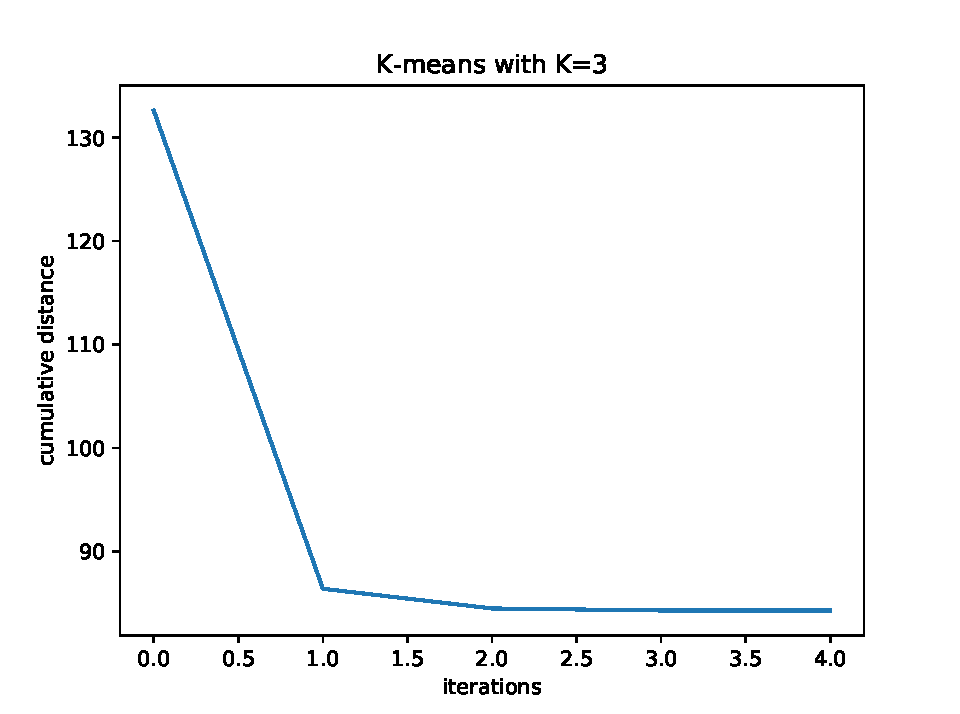
\includegraphics[width=0.6\textwidth]{./Figures/2_2_Kmeans_distance_K3}
\caption{Cumulative distance function over iterations for $K=3$ components.}
\label{2_2_Kmeans_distance}
\end{figure}

The optimisation process converges in the same number of iterations as in scenario 1 (s. \ref{2_2_Kmeans_distance} and \ref{2_1_Kmeans_distance}), much faster than the EM algorithm. One can comprehend the cluster-updates during the optimisation process visualised in figure \ref{2_2_Kmeans_iter}.

\begin{figure}[!ht]
	\makebox[\textwidth]{
	\begin{subfigure}{0.6\textwidth}
	\includegraphics[width=\textwidth]{./Figures/2_2_Kmeans_iter0}
	%\caption{Dataset}
	\end{subfigure}
	\begin{subfigure}{0.6\textwidth}
	\includegraphics[width=\textwidth]{./Figures/2_2_Kmeans_iter1}
	%\caption{$K=2$}
	\end{subfigure}
	}
	\makebox[\textwidth]{
	\begin{subfigure}{0.6\textwidth}
	\includegraphics[width=\textwidth]{./Figures/2_2_Kmeans_iter2}
	%\caption{$K=3$}
	\end{subfigure}
	\begin{subfigure}{0.6\textwidth}
	\includegraphics[width=\textwidth]{./Figures/2_2_Kmeans_converged}
	%\caption{$K=4$}
	\end{subfigure}
	}	
	\caption{Results of hard-classification during optimisation.}
	\label{2_2_Kmeans_iter}
\end{figure}

\end{document}}